\documentclass[11pt,a4paper]{article}

\usepackage[margin=1in]{geometry}
\usepackage[utf8]{inputenc}
\usepackage[T1]{fontenc}
\usepackage{lmodern}
\usepackage{microtype}
\usepackage{hyperref}
\usepackage{amsmath,amssymb,amsfonts,amsthm}
\usepackage{mathtools}
\usepackage[nameinlink,noabbrev]{cleveref}
\usepackage{booktabs}
\usepackage{array}
\usepackage{longtable}
\usepackage{enumitem}
\usepackage{siunitx}
\usepackage{listings}
\usepackage{xcolor}
\usepackage{caption}
\usepackage{subcaption}
\usepackage{float}
\usepackage{parskip}
\usepackage{tikz}
\usetikzlibrary{shapes.geometric, arrows, arrows.meta, positioning, calc, fit, backgrounds}

\tikzset{
    box/.style={rectangle, draw, rounded corners, minimum width=2.5cm, minimum height=1cm, text centered, font=\small},
    arrow/.style={thick,->,>=stealth}
}

\hypersetup{
    colorlinks=true,
    linkcolor=blue,
    urlcolor=cyan,
    citecolor=blue,
    pdftitle={InterLink: A Zero-Knowledge Atomic Cross-Chain Interoperability Protocol with Unified Liquidity and Incentive-Aligned Tokenomics},
    pdfauthor={MeridianAlgo},
    pdfsubject={Blockchain Interoperability Research Paper},
    pdflang={en}
}

\definecolor{codegreen}{rgb}{0,0.6,0}
\definecolor{codegray}{rgb}{0.5,0.5,0.5}
\definecolor{codepurple}{rgb}{0.58,0,0.82}
\definecolor{backcolour}{rgb}{0.95,0.95,0.92}

% Define Rust language for listings
\lstdefinelanguage{Rust}{
  morekeywords={abstract,as,async,await,become,box,break,const,continue,crate,do,dyn,else,enum,extern,false,fn,for,if,impl,in,let,loop,macro,match,mod,move,mut,pub,ref,return,self,Self,static,struct,super,trait,true,type,typeof,unsafe,unsized,use,virtual,where,while,yield},
  sensitive=true,
  morecomment=[l]{//},
  morecomment=[s]{/*}{*/},
  morestring=[b]",
  morestring=[b]',
}
\lstdefinestyle{mystyle}{
    backgroundcolor=\color{backcolour},
    commentstyle=\color{codegreen},
    keywordstyle=\color{magenta},
    numberstyle=\tiny\color{codegray},
    stringstyle=\color{codepurple},
    basicstyle=\ttfamily\footnotesize,
    breaklines=true,
    captionpos=b,
    keepspaces=true,
    numbers=left,
    numbersep=5pt,
    showstringspaces=false,
    tabsize=2,
    language=Rust,
    frame=single,
    framesep=5pt,
    framerule=0.5pt
}
\lstset{style=mystyle}

\setlength{\parindent}{0pt}
\setlength{\parskip}{8pt plus 2pt minus 1pt}

\title{
    \vspace{2in}
    \textbf{\Huge InterLink Protocol}\\
    \vspace{0.5in}
    \large A Zero-Knowledge Atomic Interoperability Framework\\
    \vspace{0.2in}
    \textit{Trustless. Scalable. Unified.}\\
    \vspace{1in}
    \textbf{Ishaan Manoor}\\
    MeridianAlgo Research Lab\\
    \vspace{0.1in}
    Version v1.0.0 \quad \textbullet \quad March 2026\\
    \vspace{0.1in}
    \textit{Audit-Candidate Release}\\
    \vspace{0.2in}
    {\small\url{https://github.com/MeridianAlgo/Interlink}}
}
\author{}
\date{}

\begin{document}

\begin{titlepage}
\maketitle
\end{titlepage}
\newpage

\tableofcontents
\phantomsection
\addcontentsline{toc}{section}{Abstract}
\clearpage
\begin{abstract}
 \section*{Abstract}

The blockchain ecosystem has fractured into dozens of isolated networks, each holding billions in trapped liquidity. Over \$2 billion has been stolen from cross chain bridges since 2020, exposing the fundamental weakness of trust-based interoperability. Users face a fragmented world where moving assets between chains requires trusting small committees of validators---a model that has repeatedly failed catastrophically.

This paper introduces \textbf{InterLink}, a zero knowledge cross chain protocol that replaces human trust with mathematical proof. Instead of asking ``do you trust these validators?'' InterLink asks ``does this cryptographic proof verify?'' The answer is deterministic, unforgeable, and instant.

\textbf{Core Innovation:} InterLink combines recursive zk-SNARKs (built on Halo2) with a high throughput Solana Hub to achieve what was previously considered impossible: trustless cross chain transfers with sub-minute finality and 99\% lower verification costs than traditional light clients.

\textbf{Key Results:}
\begin{itemize}[noitemsep,topsep=0pt]
    \item \textit{Security:} Cryptographic soundness ($2^{-128}$ forgery probability) vs. social consensus
    \item \textit{Performance:} 850ms proving time, 200k Solana compute units verification
    \item \textit{Scalability:} O(1) batch verification through recursive proof folding
    \item \textit{Economics:} Deflationary tokenomics with buy-back-and-burn mechanism
\end{itemize}

InterLink is not merely a bridge---it is a \textit{unified liquidity layer} that transforms the fragmented multi chain reality into a seamless, interoperable ecosystem. We present the complete protocol specification, Rust implementation details, security proofs, and economic model required for production deployment.

\vspace{0.3in}
\noindent\textbf{Keywords:} Zero-Knowledge Proofs, Recursive SNARKs, Halo2, Blockchain Interoperability, Cross-Chain Bridges, Solana, Atomic Composability, Liquidity Unification, Decentralized Finance, Cryptographic Security.
\end{abstract}

\newpage

\section*{Executive Summary}
\addcontentsline{toc}{section}{Executive Summary}

\textit{For readers who want the key takeaways without the technical deep-dive.}

\subsection*{The Problem in Plain English}

Imagine the internet, but every website runs on a different operating system that can't talk to the others. You'd need to manually copy files between computers, hoping nothing gets lost or stolen in transit. That's today's blockchain world.

We have Ethereum (the ``world computer''), Solana (the ``speed demon''), Cosmos (the ``internet of blockchains''), and dozens more. Each holds billions of dollars, but they're isolated. Moving money between them requires ``bridges''---and bridges keep getting hacked. Since 2020, hackers have stolen over \$2 billion from bridges because most rely on small groups of people to manually verify transactions. When those people make mistakes or get compromised, everyone loses money.

\subsection*{Our Solution: Math Instead of Trust}

InterLink replaces human validators with mathematical proof. Here's the simple version:

\begin{enumerate}
    \item You deposit money on Ethereum (or any supported chain).
    \item A Relayer creates a cryptographic proof (think of it as an unforgeable digital receipt that mathematically proves your deposit happened).
    \item Solana verifies the proof in milliseconds. If the math checks out, your money appears on Solana. If not, nothing happens (no theft possible).
    \item If anything goes wrong, you get an automatic refund to your original wallet.
\end{enumerate}

The key insight: \textit{you don't need to trust anyone}. You only need to trust math---and math doesn't lie, collude, or get hacked.

\subsection*{Why This Matters}

\begin{figure}[H]
\centering
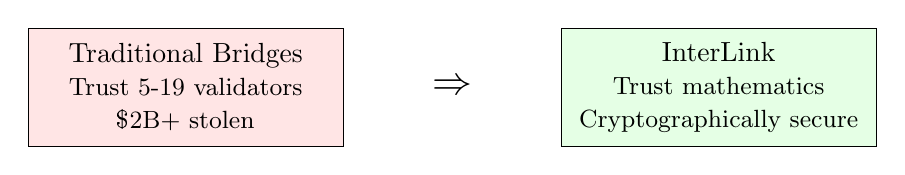
\begin{tikzpicture}[node distance=1.5cm]
    \node (oldbox) [rectangle, draw, fill=red!10, minimum width=4cm, minimum height=1.5cm, align=center] {Traditional Bridges\\{\small Trust 5-19 validators}\\{\small \$2B+ stolen}};
    \node (bigarrow) [right=1cm of oldbox, font=\Large] {$\Rightarrow$};
    \node (newbox) [rectangle, draw, fill=green!10, minimum width=4cm, minimum height=1.5cm, align=center, right=1cm of bigarrow] {InterLink\\{\small Trust mathematics}\\{\small Cryptographically secure}};
\end{tikzpicture}
\caption{The paradigm shift from trust-based to proof-based security.}
\end{figure}

\begin{itemize}
    \item For Users: Move assets across chains safely, cheaply, and quickly.
    \item For Developers: Build apps that work across multiple blockchains seamlessly.
    \item For DeFi: Unlock \$100B+ in fragmented liquidity currently trapped in isolated chains.
    \item For the Industry: End the era of catastrophic bridge hacks.
\end{itemize}

\subsection*{Business Model}

InterLink charges a small fee (0.1\%) on cross chain transfers. 40\% of fees are used to buy and burn ILINK tokens (creating scarcity), while 60\% reward the Relayers who generate proofs. This creates sustainable economics: more usage means more token burns, benefiting all stakeholders.

\subsection*{Current Status}

\begin{itemize}
    \item Now: Core cryptographic circuits in development, internal testing underway.
    \item Q4 2026: Public testnet launch with Ethereum to Solana support.
    \item Q3 2027: Mainnet launch following security audits.
    \item 2028 onwards: Expansion to 10+ chains, privacy features, institutional adoption.
\end{itemize}

\textit{The rest of this paper provides the complete technical specification for cryptographers, developers, and auditors. Non-technical readers may skip to Section~\ref{sec:tokenomics} (Tokenomics) and Section~\ref{sec:workflows} (Practical Workflows) for application-focused content.}

\newpage

\section{Introduction}
\label{sec:intro}

\subsection{A Brief History of Blockchain}
To understand why InterLink exists, we must first look at how blockchains evolved. 

In 2009, Bitcoin launched as the first successful blockchain, a decentralized ledger that allowed people to send money without a bank. Think of it like a global, unhackable spreadsheet where everyone agrees on who owns what. However, Bitcoin was designed to do just one thing: transfer its own currency.

Then came Ethereum in 2015. Ethereum introduced ``smart contracts,'' which are basically digital vending machines. You put crypto in, and if certain rules are met, the machine does something (like lending you another asset or creating a digital collectible). This spawned the world of Decentralized Finance (DeFi) and Web3.

But there was a catch. As millions of people started using Ethereum, the network got clogged. Transaction fees skyrocketed. In response, developers built \textit{new} blockchains to handle the traffic. Some, like Arbitrum or Optimism, were engineered to sit on top of Ethereum (Layer 2s). Others, like Solana, were built entirely from scratch to be incredibly fast and cheap. 

\subsection{The Protocol Chasm: Why Connecting Asymmetric Chains is Hard}
The very success of this multi chain expansion has caused a new, critical problem: fragmentation. 

Today, we have dozens of highly successful blockchains, but they don't speak the same language. Each network is like an isolated island with its own unique laws, currency, and language (or protocol). For instance, Ethereum relies on an account-based model operated by the Ethereum Virtual Machine (EVM), while Solana utilizes a highly parallelized, stateless architecture. 

Because the underlying protocols of these chains are so fundamentally different, creating a universal translator to link them together is an immense engineering challenge. Historically, there have been very few viable solutions for bridging these asymmetric environments, and almost none of them have been both secure and economically feasible at scale. If engineers wanted real security, they had to deploy heavy, data-intensive light clients onto the blockchains that simply cost too much money in transaction fees to maintain. If they wanted it to be cheap, they had to severely compromise on the mathematical security.

\subsection{The Shortcut: Vulnerable Traditional Bridges}
To bypass these economic limitations, the industry opted for a cheaper shortcut: traditional bridges. But these bridges are fundamentally archaic. 

Imagine a group of five security guards sitting in a booth between two islands. When you want to move money, you give it to the guards on island A, and they radio their friends on island B to give you a matching token. This is how most cross chain bridges work today, using what is called a multisig (multiple signatures) or an external oracle committee. 

You are forced to trust that the guards won't steal your money or get hacked. Unsurprisingly, hackers have targeted these weak points over the last few years, resulting in billions of dollars stolen. We have seen enough massive exploits to know that we need something fundamentally better than blind trust.

\subsection{Enter InterLink: Teleportation Through Math}
InterLink is our answer to the fragmentation crisis. Rather than relying on a group of human guards to verify transactions, InterLink uses pure mathematics, specifically a cutting-edge technology called Zero-Knowledge Proofs (zk-SNARKs). 

For a normal user, you can think of InterLink as a secure teleporter. When you want to move an asset or data from Ethereum to Solana, our system takes a cryptographic snapshot (a proof) of your action. This proof is a mathematical guarantee that the action happened. We then send this tiny proof to the Solana network, which acts as our central Hub. 

Because we use math instead of trusted humans, no one can fake a transaction. If the math checks out, the transaction executes automatically. If it doesn't, nothing happens. This removes the risk of human error or malicious groups stealing funds.

\subsection{Competitive Landscape}

To contextualize InterLink's position in the interoperability space, we provide a qualitative comparison with leading cross chain protocols. This analysis focuses on key dimensions: security model, verification cost, latency, finality guarantees, and capital efficiency.

\begin{table}[H]
\centering
\begin{tabular}{@{}lccc@{}}
\toprule
Protocol & Security Model & Proposed Verification Cost & Proposed Latency \\
\midrule
LayerZero & Multisig + DVN & Medium & 5-20 min \\
Axelar & Multisig Guardians & Low & 1-5 min \\
Wormhole & Multisig Guardians & Low & 1-5 min \\
IBC & Light Clients & High & 10-30 min \\
Chainlink CCIP & Oracle Networks & Medium & 5-15 min \\
InterLink & zk-SNARK Proofs & Low (O(1)) & 1-5 min \\
\bottomrule
\end{tabular}
\caption{Competitive Comparison: Part 1 (Proposed) - Security, Cost, and Latency.}
\end{table}

\begin{table}[H]
\centering
\begin{tabular}{@{}lcc@{}}
\toprule
Protocol & Finality & Capital Efficiency \\
\midrule
LayerZero & Probabilistic & High \\
Axelar & Probabilistic & Medium \\
Wormhole & Probabilistic & High \\
IBC & Deterministic & Low \\
Chainlink CCIP & Probabilistic & High \\
InterLink & Deterministic & Very High \\
\bottomrule
\end{tabular}
\caption{Competitive Comparison: Part 2 - Finality and Efficiency.}
\end{table}

\subsection{The Genesis of InterLink: A Proposal for Unification}
We propose InterLink as a solution to the interoperability trilemma (scalability, security, and generality) without relying on weak trust assumptions. The trajectory is not simply many chains, but a cross chain-native environment in which value and application state can move and compose safely across heterogeneous runtimes.

Existing solutions ask users to trust a third party. InterLink instead aims to reduce trust to verification. By leveraging zero knowledge proofs (zk-SNARKs), specifically circuits built with the halo2 proving system, InterLink is designed to let one environment cryptographically validate key state-transition claims originating from another. In the intended flow, a relayer proves that a transaction occurred on a source chain, and the Solana Hub verifies the proof efficiently. This removes the need for trusted validators: if the proof is valid, the event is valid for cross chain execution.

InterLink is not envisioned solely as a message-passing protocol; it is being built as a liquidity unification layer. By using Solana as a high performance execution hub, the protocol coordinates cross chain intents and routes execution through a shared liquidity surface. The target user experience is atomic intent execution (for example, swapping a token on Ethereum for a token on Cosmos) where safety (no asset loss) is cryptographically guaranteed by ZK proofs, while the Hub manages the settlement across participating chains.

We have chosen a modular architecture that respects the sovereignty of each chain while leveraging Solana's throughput for coordination. Proof generation happens off-chain via a decentralized network of relayers, while verification and state progression occur on-chain. This separation keeps the verification path succinct while pushing expensive computation to the edge, enabling high cross chain throughput without congesting source or destination chains.

\section{Core Definitions}
\label{sec:definitions}

To ensure clarity throughout this technical compendium, we define the following core terms and actors used throughout the InterLink ecosystem.

\begin{description}
    \item[The Hub (Solana):] The global coordination layer and state manager. It is implemented on Solana and is responsible for verifying ZK proofs from connected chains and coordinating cross chain state transitions.
    \item[The Spoke (External Chain):] Any blockchain network connected to the InterLink Hub, such as Ethereum, Arbitrum, or the Cosmos Hub.
    \item[Gateway Contract:] A set of smart contracts deployed on a Spoke chain that escrows assets, emits canonical events, and executes verified messages.
    \item[Relayer:] An off-chain node that observes Gateway events on Spoke chains, generates zk-SNARK proofs about those events, and submits proofs and public inputs to the Hub.
    \item[zk-SNARK:] (Zero-Knowledge Succinct Non-Interactive Argument of Knowledge) A cryptographic proof that convinces a verifier that a statement is true without revealing the underlying private inputs beyond what is implied by correctness.
    \item[KZG (Kate-Zaverucha-Goldberg):] A polynomial commitment scheme that allows a prover to commit to a polynomial and later prove evaluations without revealing the entire polynomial. Used for the final outer proof submitted to Ethereum, providing constant-size proofs (48 bytes) and constant-time verification, though requiring a trusted setup.
    \item[Recursive Proof:] A proof that verifies another proof. In InterLink, many transaction proofs are aggregated (``folded'') into a single recursive proof to reduce amortized on-chain verification costs.
    \item[Program Derived Address (PDA):] A Solana-specific construct where an address is deterministically derived from a program ID and seed values. InterLink uses PDAs to represent accounts and vaults on Solana without requiring corresponding private keys.
    \item[Atomic-Intent Execution:] The property that a multi-step, cross chain operation is initiated as a single atomic intent, where safety (no lost funds) is guaranteed by ZK proofs, and liveness is handled by relayer incentives.
    \item[Liveness:] The guarantee that the system continues to make progress (i.e., messages are eventually processed) even under partial faults.
    \item[Safety:] The cryptographic guarantee that the system never accepts an invalid state transition (e.g., minting assets without a proven deposit).
\end{description}

\section{Preliminaries}
\label{sec:prelim}

To provide a rigorous foundation for the InterLink Protocol, we first establish the mathematical and cryptographic primitives on which the system is built. This section summarizes the key concepts and the concrete choices we make for curves, proving systems, and runtime environments.

\subsection{The Concept of Zero-Knowledge}
Before diving into the technicalities of SNARKs, it is helpful to build intuition for what a zero knowledge proof guarantees and what it explicitly does not.

\subsubsection{Intuition: Interactive Zero-Knowledge Proofs}

Zero-knowledge proofs allow a prover to convince a verifier of a statement's truth without revealing the underlying evidence. The classic protocol works as follows:
\begin{enumerate}
    \item Peggy enters the cave and randomly chooses path A or path B while Victor waits outside.
    \item Victor then enters and requests that Peggy exit via path A (or path B).
    \item If Peggy knows the password, she can always comply by opening the door if needed.
    \item If Peggy does not know the password, she has a 50\% chance of being on the wrong side and failing the challenge.
\end{enumerate}

Repeating this test $n$ times reduces the probability of cheating to $2^{-n}$. For example, with $n=40$, the cheating probability is negligible. Victor becomes convinced that Peggy knows the password, yet learns nothing about the password itself.

\subsection{zk-SNARKs: A Technical Deep Dive}

InterLink utilizes zk-SNARKs (Zero-Knowledge Succinct Non-Interactive Arguments of Knowledge). Before diving into the technical details, let's build intuition for what makes SNARKs so powerful.

\subsubsection{Why SNARKs Change Everything}

Traditional verification requires the verifier to redo all the work. If you want to prove a Sudoku is solved correctly, the verifier must check all 81 cells. With a SNARK, you generate a tiny ``proof'' (a few hundred bytes) that convinces any verifier---instantly---that you know a valid solution, \textit{without showing the solution itself}.

\begin{figure}[H]
\centering
\resizebox{0.9\textwidth}{!}{
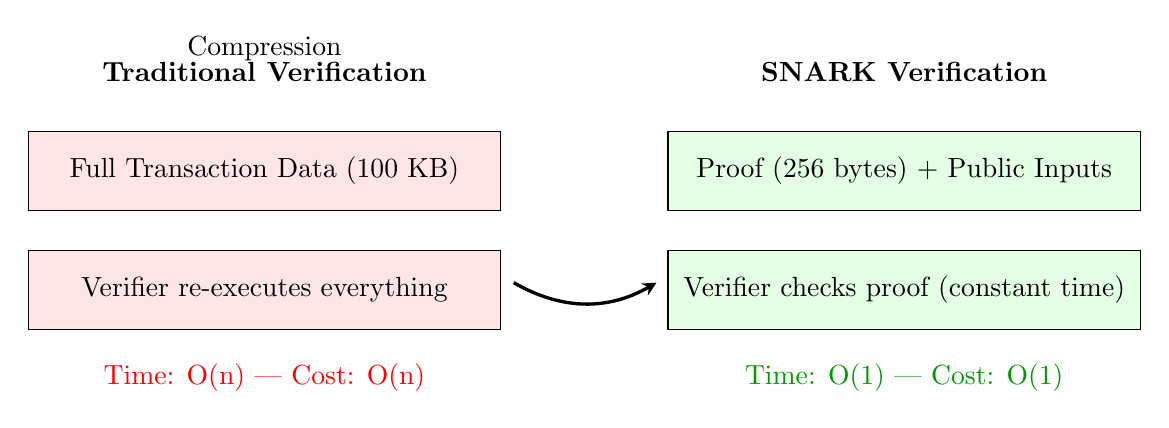
\begin{tikzpicture}[node distance=1.5cm, auto, >=stealth]
    % Traditional Verification
    \node (trad_title) [font=\bfseries] {Traditional Verification};
    \node (trad_data) [rectangle, draw, fill=red!10, below=0.5cm of trad_title, minimum width=6cm, minimum height=1cm] {Full Transaction Data (100 KB)};
    \node (trad_verify) [rectangle, draw, fill=red!10, below=0.5cm of trad_data, minimum width=6cm, minimum height=1cm] {Verifier re-executes everything};
    \node (trad_time) [below=0.3cm of trad_verify, text=red] {Time: O(n) --- Cost: O(n)};

    % SNARK Verification
    \node (snark_title) [font=\bfseries, right=4cm of trad_title] {SNARK Verification};
    \node (snark_proof) [rectangle, draw, fill=green!10, below=0.5cm of snark_title, minimum width=6cm, minimum height=1cm] {Proof (256 bytes) + Public Inputs};
    \node (snark_verify) [rectangle, draw, fill=green!10, below=0.5cm of snark_proof, minimum width=6cm, minimum height=1cm] {Verifier checks proof (constant time)};
    \node (snark_time) [below=0.3cm of snark_verify, text=green!60!black] {Time: O(1) --- Cost: O(1)};

    % Arrow between them
    \draw [->, very thick, bend right] ($(trad_time.east)+(1cm,1.2cm)$) to ($(snark_time.west)+(-1cm,1.2cm)$) node[midway, above] {Compression};
\end{tikzpicture}
}
\caption{SNARKs compress verification from linear to constant time. The verifier never sees the original data---only the proof.}
\end{figure}

For InterLink, this means: instead of Solana needing to verify 100 Ethereum blocks (impossible!), it verifies a single 256-byte proof in milliseconds.

\subsubsection{The Five Properties of zk-SNARKs}

The acronym captures five key properties:

\begin{description}
    \item[Zero-Knowledge:] The verifier learns nothing about the prover's private inputs (the witness) beyond the fact that the statement is true. In InterLink, this means the Hub can learn that ``Transaction X occurred on Ethereum'' without ingesting Ethereum's full state or history.
    
    \item[Succinct:] Proofs are compact and efficient to verify. In practice, proof sizes can be constant or logarithmic in the statement size, and verification can complete in milliseconds. This property is essential for on-chain verification, where storage and compute are constrained.
    
    \item[Non-Interactive:] The prover produces a proof once, and anyone can verify it later without additional interaction. This is typically achieved via the Fiat--Shamir heuristic, which replaces the verifier's random challenges with hash-derived challenges.
    
    \item[Argument:] The soundness guarantee holds against computationally bounded adversaries (i.e., those unable to break the underlying hardness assumptions within feasible resources). For blockchain settings, this is the relevant security model.
    
    \item[of Knowledge:] The proof implies that the prover actually \emph{knows} a valid witness, not merely that one exists in principle.
\end{description}

\subsection{Elliptic Curve Cryptography (ECC)}
InterLink selects specific elliptic curves to balance practical on-chain verification (especially on the EVM) with efficient recursive proof composition inside Halo2.

\subsubsection{BN254 (Alt-Bn128)}
For interoperability with the Ethereum Virtual Machine (EVM), we utilize the BN254 curve. BN254 is pairing-friendly and defined over a finite field $\mathbb{F}_q$, enabling efficient bilinear pairings $e: \mathbb{G}_1 \times \mathbb{G}_2 \rightarrow \mathbb{G}_T$. These pairings are a core primitive for verifying KZG commitments on-chain.
$$ y^2 = x^3 + 3 \mod q $$
Ethereum includes dedicated precompiled contracts (0x06, 0x07, 0x08) for BN254 operations, which makes verification substantially more gas-efficient than generic elliptic-curve arithmetic.

\subsubsection{Pallas and Vesta (The Pasta Curves)}
For recursive proof generation inside the Relayer Network, we employ the Pallas and Vesta curves (the Pasta curves). These curves were specifically designed for recursive proof composition and form a cycle: the scalar field of Pallas is the base field of Vesta, and vice versa.

The Pasta curves are defined as:
\begin{itemize}
    \item Pallas: $y^2 = x^3 + 5$ over the field $\mathbb{F}_p$ where $p = 2^{254} + 45560315531419706090280762371685220353$
    \item Vesta: $y^2 = x^3 + 5$ over the field $\mathbb{F}_q$ where $q = 2^{254} + 45560315531506369815346746415080538113$
\end{itemize}

This cycle property allows a proof generated over one curve to be verified efficiently inside a circuit over the other, avoiding the heavy overhead of non-native (wrong-field) arithmetic. This choice is central to InterLink's Halo2 recursion strategy.

\subsection{Polynomial Commitment Schemes (PCS)}
A polynomial commitment scheme (PCS) allows a prover to commit to a polynomial $P(X)$ and later prove evaluations of the form $P(z)=y$ without revealing the entire polynomial. InterLink uses a hybrid approach combining two complementary schemes.

\subsubsection{IPA (Inner Product Argument)}
IPA is used for internal inner proofs inside the recursive proving pipeline.
\begin{itemize}
    \item Pros: Transparent (no trusted setup), relies only on discrete log hardness.
    \item Cons: $O(\log n)$ verification time (slower than KZG).
\end{itemize}

\subsubsection{KZG (Kate-Zaverucha-Goldberg)}
KZG is used for the final outer proof submitted to Ethereum.
\begin{itemize}
    \item Pros: Constant size proofs (48 bytes), constant time verification.
    \item Cons: Requires a Trusted Setup (Structured Reference String).
\end{itemize}

InterLink uses IPA for recursion and accumulation, then a final wrap (e.g., into KZG or Groth16) to minimize on-chain verification cost.

\subsection{Solana Runtime (Sealevel)}
Solana's runtime model (Sealevel) differs fundamentally from EVM-based chains.
\begin{itemize}
    \item \textit{Stateless Execution:} Programs (smart contracts) are stateless; state is stored in separate "Accounts."
    \item \textit{Parallelism:} Transactions specify all accounts they will read or write upfront. This allows the runtime to schedule non-overlapping transactions in parallel.
    \item \textit{PDAs (Program Derived Addresses):} Addresses deterministically derived from a program ID and seeds (e.g., \texttt{hash("user\_vault", user\_pubkey)}). This allows us to map a user's Ethereum address to a specific Solana account without needing a private key for that account.
\end{itemize}

\section{System Architecture}
\label{sec:arch}

Before diving into components, here's the complete picture of how InterLink moves value across chains:

\begin{figure}[H]
\centering
\resizebox{\textwidth}{!}{
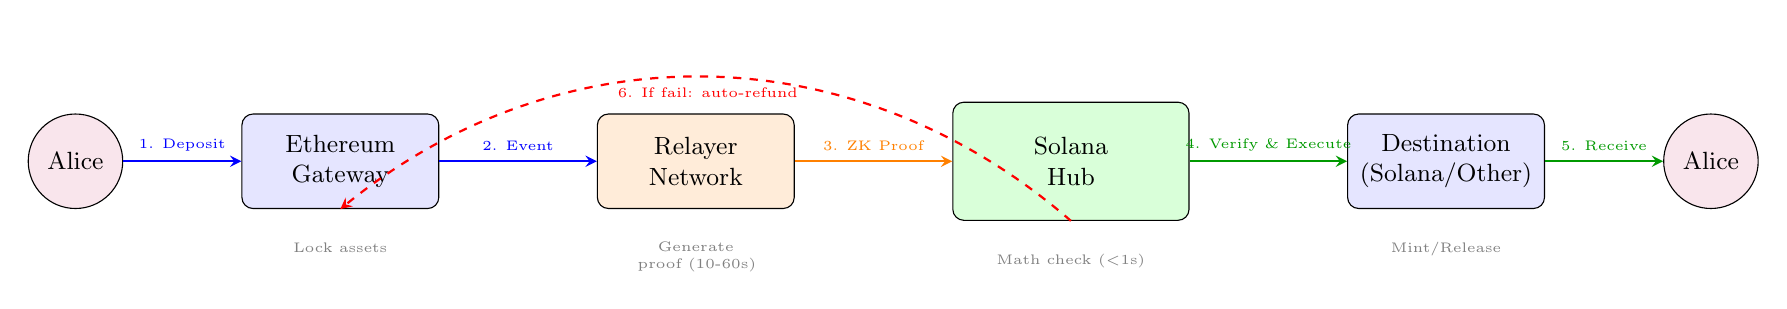
\begin{tikzpicture}[
    node distance=1.2cm,
    auto,
    >=stealth,
    userbox/.style={circle, draw, fill=purple!10, minimum size=1.2cm, font=\small},
    chainbox/.style={rectangle, draw, rounded corners, fill=blue!10, minimum width=2.5cm, minimum height=1.2cm, font=\small, align=center},
    hubbox/.style={rectangle, draw, rounded corners, fill=green!15, minimum width=3cm, minimum height=1.5cm, font=\small, align=center},
    relayerbox/.style={rectangle, draw, rounded corners, fill=orange!15, minimum width=2.5cm, minimum height=1.2cm, font=\small, align=center},
    stepnum/.style={circle, draw, fill=white, minimum size=0.5cm, font=\tiny\bfseries}
]

    % User
    \node (user) [userbox] {Alice};

    % Source Chain (Ethereum)
    \node (eth) [chainbox, right=1.5cm of user] {Ethereum\\Gateway};

    % Relayer Network
    \node (relayer) [relayerbox, right=2cm of eth] {Relayer\\Network};

    % Solana Hub
    \node (hub) [hubbox, right=2cm of relayer] {Solana\\Hub};

    % Destination Chain (could be same as hub or different)
    \node (dest) [chainbox, right=2cm of hub] {Destination\\(Solana/Other)};

    % User wallet on destination
    \node (user2) [userbox, right=1.5cm of dest] {Alice};

    % Flow arrows with numbered steps
    \draw [->, thick, blue] (user) -- (eth) node[midway, above, font=\tiny] {1. Deposit};
    \draw [->, thick, blue] (eth) -- (relayer) node[midway, above, font=\tiny] {2. Event};
    \draw [->, thick, orange] (relayer) -- (hub) node[midway, above, font=\tiny] {3. ZK Proof};
    \draw [->, thick, green!60!black] (hub) -- (dest) node[midway, above, font=\tiny] {4. Verify \& Execute};
    \draw [->, thick, green!60!black] (dest) -- (user2) node[midway, above, font=\tiny] {5. Receive};

    % Time annotations below
    \node [below=0.3cm of eth, font=\tiny, text=gray, align=center] {Lock assets};
    \node [below=0.3cm of relayer, font=\tiny, text=gray, align=center, text width=1.8cm] {Generate proof (10-60s)};
    \node [below=0.3cm of hub, font=\tiny, text=gray, align=center] {Math check ($<$1s)};
    \node [below=0.3cm of dest, font=\tiny, text=gray, align=center] {Mint/Release};

    % Failure path
    \draw [->, thick, dashed, red] (hub.south) to[bend right=40] node[below, font=\tiny, text=red] {6. If fail: auto-refund} (eth.south);

\end{tikzpicture}
}
\caption{Complete InterLink transaction flow. Alice deposits on Ethereum, Relayers generate ZK proofs, the Solana Hub verifies mathematically, and assets appear at the destination. If anything fails, automatic refund to Alice.}
\end{figure}

\textbf{Key Insight:} Notice there's no ``trusted validator'' step. The Hub doesn't \textit{ask} anyone if the transaction is valid---it \textit{proves} it mathematically. This is the fundamental difference from traditional bridges.

\subsection{The Hub-and-Spoke Topology}

InterLink employs a hub-and-spoke network topology to minimize complexity and maximize scalability. 

\begin{figure}[H]
\centering
\resizebox{0.9\textwidth}{!}{
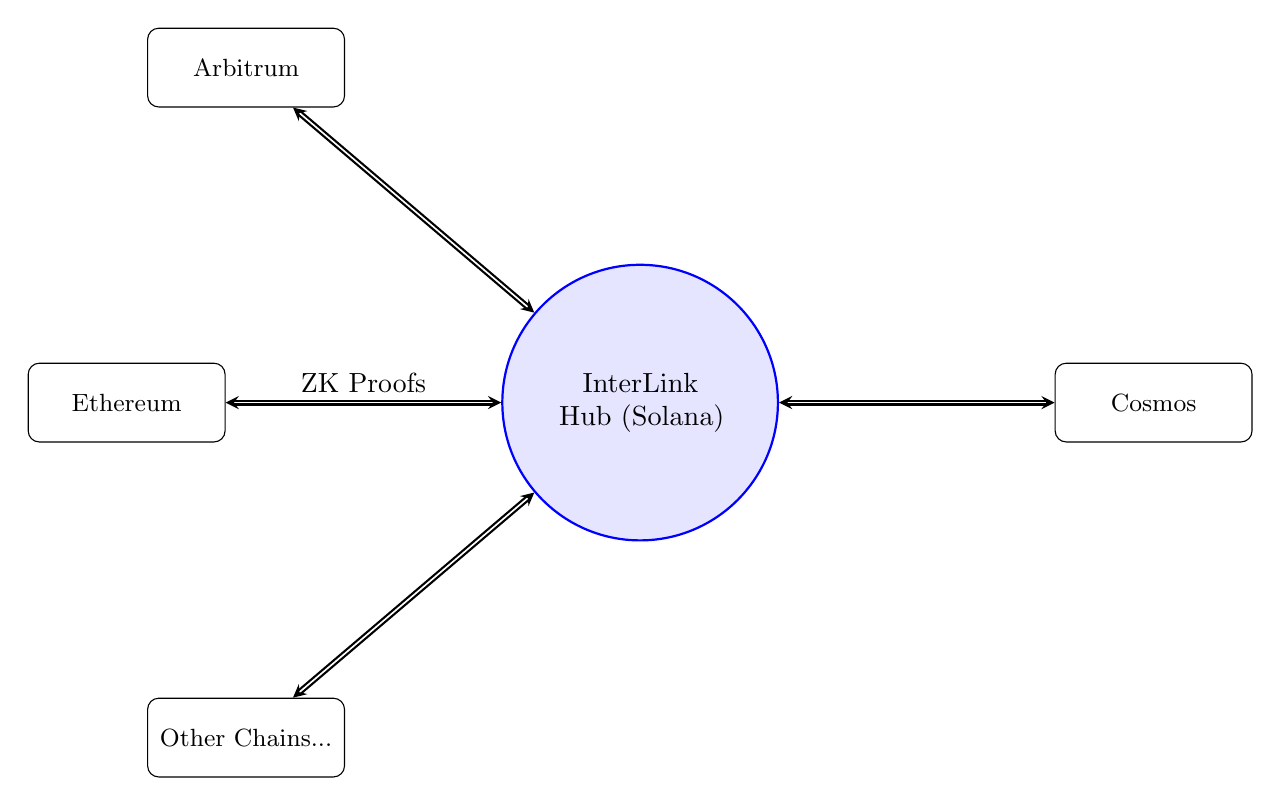
\begin{tikzpicture}[node distance=3cm, auto, >=stealth]
    \node (hub) [circle, draw=blue, fill=blue!10, thick, minimum size=3.5cm, text width=2.5cm, align=center] {InterLink Hub (Solana)};
    \node (eth) [box, left = 3.5cm of hub] {Ethereum};
    \node (arb) [box, above left = 2.5cm and 2.5cm of hub] {Arbitrum};
    \node (cos) [box, right = 3.5cm of hub] {Cosmos};
    \node (sol) [box, below left = 2.5cm and 2.5cm of hub] {Other Chains...};
    
    \draw [double, <->, thick] (hub) -- (eth) node [midway, above, sloped] {ZK Proofs};
    \draw [double, <->, thick] (hub) -- (arb);
    \draw [double, <->, thick] (hub) -- (cos);
    \draw [double, <->, thick] (hub) -- (sol);
\end{tikzpicture}
}
\caption{Connecting chains through a central Solana Hub.}
\end{figure}


\subsubsection{Topology Description}
In the InterLink hub-and-spoke model:
\begin{itemize}
    \item The Hub (Solana): Serves as the global clearinghouse and state manager, implemented on the Solana blockchain. All cross chain messages are routed through this central hub, which verifies zk-SNARK proofs from connected chains and coordinates cross chain state transitions.
    \item The Spokes (External Chains): Represent individual blockchain networks connected to the InterLink Hub, such as Ethereum, Arbitrum, Optimism, Cosmos Hub, and Sui. Each spoke maintains its own Gateway contract for interaction with the hub.
\end{itemize}

This design yields O(N) connection complexity, far superior to the O(N²) complexity of pairwise bridges. The notation O(N) describes the computational complexity, meaning the number of connections grows linearly with the number of chains. In contrast, O(N²) means the connections grow quadratically (if you have 10 chains, you need 45 pairwise connections; with 100 chains, you need 4,950 connections). Adding a new chain requires only establishing a connection to the Solana Hub, rather than creating N-1 new bridge connections.

\subsubsection{Topology Advantages and Trade-offs}

Advantages:
\begin{itemize}
    \item Scalability: New chains can be added without modifying existing spoke implementations, enabling rapid ecosystem expansion.
    \item Consistency: All cross chain operations flow through a single verification layer, ensuring uniform security guarantees.
    \item Efficiency: Shared liquidity and routing logic reduce redundant implementations across chains.
    \item Simplicity: Centralized coordination simplifies protocol upgrades and governance decisions.
\end{itemize}

Trade-offs:
\begin{itemize}
    \item Single Point of Coordination: While not a single point of failure (due to cryptographic verification), the hub becomes a critical coordination point.
    \item Hub Performance Dependency: Cross-chain throughput is limited by the hub's capacity, though Solana's high performance mitigates this concern.
\end{itemize}

\subsubsection{Example: Cross-Chain Message Routing (The Airport Analogy)}
To understand how Hub-and-Spoke routing works in practice, imagine the Solana Hub as a massive international airport terminal, and the spokes (Ethereum, Arbitrum, etc.) as smaller regional airports. 

If you want to fly from a small regional airport in Texas (Ethereum) to a small regional airport in Alaska (Arbitrum), you don't take a direct flight. That would require building direct flight paths between every single small airport in the world (O(N²) complexity, typical of older bridges). 

Instead, you take a flight to a massive central Hub, like Chicago O'Hare (Solana). 

Consider a user sending 1,000 USDC from Ethereum to Arbitrum:
\begin{enumerate}
    \item \textbf{Departure (Ethereum Gateway):} The user deposits 1,000 USDC into the Ethereum "Regional Airport" gateway. The Relayers take a snapshot of the receipt (generating the ZK-SNARK proof) and put it on the digital airplane.
    \item \textbf{The Hub (Solana):} The proof lands at the Solana Hub. The Hub mathematically verifies the receipt in milliseconds. Because it acts as the central router, it immediately reads that the final destination is Arbitrum and approves the connecting flight.
    \item \textbf{Arrival (Arbitrum Gateway):} The Hub sends the verified release command to Arbitrum. The Arbitrum Gateway opens its vault and hands the user their 1,000 USDC.
\end{enumerate}

If the destination airport is closed or the flight fails, the Hub easily routes your refund back to the starting point. This centralized "air traffic control" enables sophisticated features like atomic multi chain operations and unified liquidity management, all while remaining 100\% mathematically secure.

\subsection{Detailed Component Breakdown}

\subsubsection{Source Chain Gateway (The Spoke)}

The Gateway contract represents InterLink's presence on each connected blockchain. It serves as the secure interface between the external chain and the InterLink Hub, handling asset custody, event emission, and verified message execution.

\subsubsection*{Core Functions}

Asset Custody: The Gateway maintains a secure vault for escrowed assets. When users initiate cross chain transfers, their tokens are locked in this vault until the destination chain confirms successful execution.

Event Emission: The Gateway emits standardized events that Relayers monitor. These events contain all necessary information for proof generation, including:
\begin{itemize}
    \item Transaction hash and block number
    \item Asset amount and recipient address  
    \item Destination chain identifier
    \item Message payload hash
\end{itemize}

Message Ingestion: Upon receiving verified proofs from the Hub, the Gateway executes the intended operations, such as releasing escrowed assets or executing arbitrary logic.

\subsubsection*{Security Architecture}

Safety Module: Each Gateway includes a Guardian role controlled by the InterLink DAO. In emergency situations, the Guardian can:
\begin{itemize}
    \item Pause all Gateway operations
    \item Authorize emergency withdrawals
    \item Update contract parameters
\end{itemize}

Replay Protection: Gateways maintain sequence numbers and message hashes to prevent duplicate executions, ensuring each cross chain message is processed exactly once.

\subsubsection*{Example: Ethereum Gateway Operation (The Lockbox Analogy)}

Consider Alice depositing 1 ETH to bridge to Solana. For a normal user, you can think of the Gateway like a high-security lockbox that holds funds securely while the mathematical proofs travel across the internet. 

When Alice locks her ETH, the lockbox effectively shouts to the surrounding network: "Hey, someone just locked 1 ETH for a ticket to Solana!" This public shout is what the Relayer network listens for.

\begin{lstlisting}[language=Java, caption={Ethereum Gateway Deposit Function}]
function deposit(
    address recipient,
    uint256 amount,
    uint16 destinationChain
) external payable {
    require(msg.value == amount, "Incorrect ETH amount");
    
    // Lock ETH in vault
    vault.deposit{value: amount}();
    
    // Emit canonical event for Relayers
    emit MessagePublished(
        sequenceNumber: ++seqNum,
        sender: msg.sender,
        recipient: recipient,
        amount: amount,
        destinationChain: destinationChain,
        payload: abi.encode(recipient, amount)
    );
}
\end{lstlisting}

When the Hub verifies the proof and sends confirmation, the Gateway on Solana (destination) mints wrapped ETH to Alice's address.

\subsubsection{The Relayer Network (The Transport)}

The Relayer Network forms the critical transport layer of InterLink, consisting of a decentralized set of off-chain nodes that observe, prove, and relay cross chain messages. 

\begin{figure}[H]
\centering
\resizebox{0.85\textwidth}{!}{
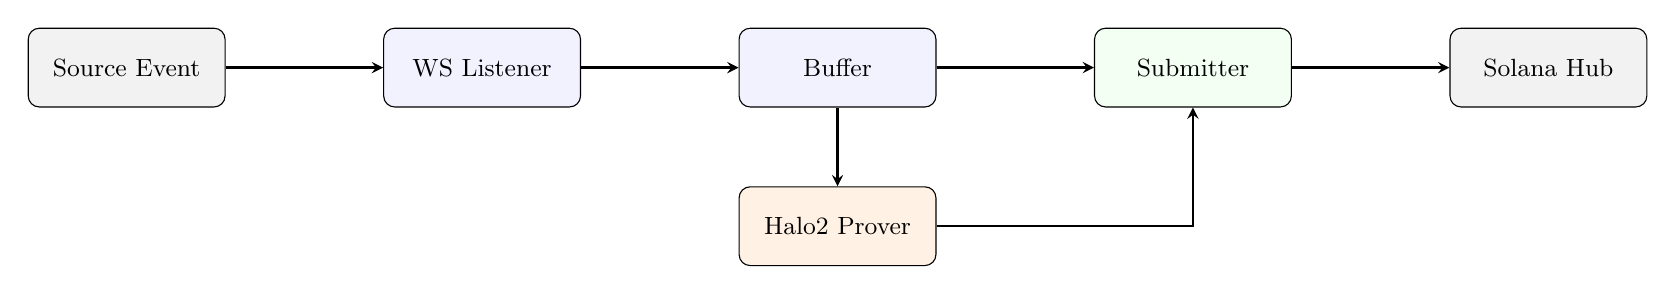
\begin{tikzpicture}[node distance=2cm, auto, >=stealth]
    \node (src) [box, fill=gray!10] {Source Event};
    \node (listen) [box, fill=blue!5, right=of src] {WS Listener};
    \node (buffer) [box, fill=blue!5, right=of listen] {Buffer};
    \node (prover) [box, fill=orange!10, below=1cm of buffer] {Halo2 Prover};
    \node (submit) [box, fill=green!5, right=of buffer] {Submitter};
    \node (hub) [box, fill=gray!10, right=of submit] {Solana Hub};
    
    \draw [arrow] (src) -- (listen);
    \draw [arrow] (listen) -- (buffer);
    \draw [arrow] (buffer) -- (submit);
    \draw [arrow] (buffer) -- (prover);
    \draw [arrow] (prover) -| (submit);
    \draw [arrow] (submit) -- (hub);
\end{tikzpicture}
}
\caption{How relayers process and prove messages.}
\end{figure}


\subsubsection*{Component Architecture}

Listener Component: Maintains persistent WebSocket connections to archive nodes of supported chains. The Listener:
\begin{itemize}
    \item Subscribes to Gateway contract events using standardized filters
    \item Buffers events in memory for processing
    \item Handles connection failures and chain reorganizations
    \item Forwards events to the Prover component via internal channels
\end{itemize}

Prover Engine: The computational core that generates zk-SNARK proofs. Built with the Halo2 proving system, it:
\begin{itemize}
    \item Fetches complete transaction data and Merkle proofs from archive nodes
    \item Constructs Halo2 circuits for transaction inclusion and consensus verification
    \item Generates succinct proofs that compress gigabytes of chain data into ~100 bytes
    \item Aggregates multiple proofs into recursive structures for efficiency
\end{itemize}

Submitter Component: Handles interaction with the Solana Hub:
\begin{itemize}
    \item Monitors mempool for optimal gas conditions
    \item Batches proofs for cost amortization
    \item Implements retry logic for failed submissions
    \item Tracks proof confirmations and collects rewards
\end{itemize}

\subsubsection*{Operational Workflow}

A Relayer processes a cross chain message through these stages:

\begin{enumerate}
    \item Event Detection: Listener detects Gateway deposit event
    \item Finality Waiting: Waits for source chain finality (12-15 minutes on Ethereum)
    \item Witness Collection: Fetches Merkle proof and block headers from archive node
    \item Proof Generation: Constructs and solves Halo2 circuits
    \item Submission: Posts proof to Solana Hub with optimal timing
    \item Reward Collection: Receives ILINK rewards for successful relay
\end{enumerate}

\subsubsection*{Incentive Structure}

Relayers earn ILINK tokens through a dual mechanism:
\begin{itemize}
    \item Base Rewards: Fixed ILINK payment per successful message relay
    \item Burn Participation: Share of tokens burned from user fees
    \item Staking Requirement: Must stake 100,000 ILINK minimum to participate
    \item Slashing: Invalid proofs result in stake reduction and burns
\end{itemize}

\subsubsection*{Example: Relayer Processing a Deposit (The Digital Notary)}

Consider Bob's Relayer processing Alice's ETH deposit. You can imagine a Relayer as a hyper-fast digital notary. The notary's job is not to hold or move the money, but strictly to gather the evidence, stamp it with an unforgeable mathematical seal (the Zero-Knowledge Proof), and hand it directly to the Solana Hub for final execution.

\begin{lstlisting}[language=Rust, caption={Relayer Event Processing Flow}]
async fn process_deposit_event(event: DepositEvent) {
    // 1. Wait for finality
    wait_for_finality(event.block_number, Chain::Ethereum).await?;
    
    // 2. Fetch witness data
    let proof = eth_client.get_proof(event.tx_hash, event.slot).await?;
    let headers = eth_client.get_block_headers(event.block_number).await?;
    
    // 3. Generate proof
    let circuit = DepositCircuit::new(event, proof, headers);
    let (proof, public_inputs) = generate_proof(circuit)?;
    
    // 4. Submit to Solana
    let tx = solana_client.submit_proof(proof, public_inputs).await?;
    
    // 5. Monitor and claim rewards
    wait_for_confirmation(tx).await?;
    claim_relayer_rewards(event.sequence).await?;
}
\end{lstlisting}

This decentralized network ensures no single entity can censor cross chain messages, while economic incentives align Relayers with protocol success.

\subsubsection{The Solana Execution Hub (The Core)}

The Solana Execution Hub serves as InterLink's central nervous system, implemented as an Anchor program on Solana. It coordinates all cross chain operations, verifies proofs, manages global state, and executes complex multi chain logic.

\subsubsection*{Core Components}

Verifier Contract: The cryptographic heart of the Hub, containing pre-deployed verification keys for all supported proof circuits. It performs:
\begin{itemize}
    \item BN254 pairing checks for KZG proofs from EVM chains
    \item Custom verification logic for IPA-based recursive proofs
    \item Batch verification of multiple aggregated proofs
\end{itemize}

State Registry: A comprehensive mapping system that tracks cross chain message state:
\begin{itemize}
    \item \texttt{chain\_id $\rightarrow$ sequence\_number}: Tracks latest processed message per chain
    \item \texttt{message\_hash $\rightarrow$ status}: Records execution status (pending, executed, failed)
    \item \texttt{user\_address $\rightarrow$ vault\_pda}: Maps user addresses to their Solana vault accounts
\end{itemize}

Liquidity Management Engine: Implements sophisticated AMM logic for cross chain swaps:
\begin{itemize}
    \item Concentrated liquidity pools with dynamic fee tiers
    \item Multi-hop routing across different token pairs
    \item Slippage protection and price impact calculations
    \item Integration with Jupiter aggregator for optimal execution
\end{itemize}

Message Dispatcher: Handles outbound cross chain communications:
\begin{itemize}
    \item Queues messages for destination chains
    \item Generates proofs for reverse-direction messages (refunds/failures)
    \item Coordinates with Relayer Network for message delivery
\end{itemize}

\subsubsection*{Verification Process}

When a Relayer submits a proof to the Hub, the verification follows this sequence:

\begin{enumerate}
    \item Input Validation: Check proof format and public inputs
    \item Circuit Verification: Execute elliptic curve operations to validate the SNARK
    \item State Transition: Update sequence numbers and message status
    \item Execution Trigger: Invoke destination logic (minting, swapping, etc.)
\end{enumerate}

\subsubsection*{Example: Hub Processing a Cross-Chain Swap}

Consider Alice swapping 1 ETH on Ethereum for USDC on Solana:

\begin{lstlisting}[language=Rust, caption={Solana Hub Verification and Execution}]
#[derive(Accounts)]
pub struct ProcessCrossChainSwap<'info> {
    #[account(mut)]
    pub verifier: Account<'info, VerifierState>,
    #[account(mut)]
    pub user_vault: Account<'info, TokenAccount>,
    #[account(mut)]
    pub liquidity_pool: Account<'info, LiquidityPool>,
    pub token_program: Program<'info, Token>,
}

pub fn process_swap(
    ctx: Context<ProcessCrossChainSwap>,
    proof: Vec<u8>,
    public_inputs: PublicInputs,
    amount_in: u64,
    min_amount_out: u64
) -> Result<()> {
    // 1. Verify the zk-SNARK proof
    let is_valid = verifier::verify_proof(&proof, &public_inputs)?;
    require!(is_valid, ErrorCode::InvalidProof);
    
    // 2. Update sequence number for Ethereum
    let mut verifier = &mut ctx.accounts.verifier;
    require!(
        public_inputs.sequence > verifier.last_eth_sequence,
        ErrorCode::OutOfOrderMessage
    );
    verifier.last_eth_sequence = public_inputs.sequence;
    
    // 3. Mint wrapped ETH to temporary vault
    token::mint_to(
        ctx.accounts.mint_weth.clone(),
        ctx.accounts.temp_vault.to_account_info(),
        amount_in
    )?;
    
    // 4. Execute swap through liquidity pool
    let swap_result = execute_swap(
        &ctx.accounts.liquidity_pool,
        amount_in,
        min_amount_out,
        ctx.accounts.user_vault.to_account_info()
    )?;
    
    // 5. Emit success event
    emit!(SwapExecuted {
        user: ctx.accounts.user_vault.owner,
        amount_in,
        amount_out: swap_result.amount_out,
        source_chain: Chain::Ethereum,
    });
    
    Ok(())
}
\end{lstlisting}

\begin{lstlisting}[language=Rust, caption={Execute Swap in Liquidity Pool}]
fn execute_swap(
    pool: &mut LiquidityPool,
    amount_in: u64,
    min_amount_out: u64,
    user_account: &Pubkey,
) -> Result<SwapResult, Error> {
    // Calculate swap output using constant product formula
    let reserve_in = pool.reserve_a;
    let reserve_out = pool.reserve_b;
    let amount_out = (amount_in as u128 * reserve_out as u128) / (reserve_in as u128 + amount_in as u128);
    
    require!(amount_out >= min_amount_out, ErrorCode::SlippageExceeded);
    
    // Update reserves
    pool.reserve_a += amount_in;
    pool.reserve_b -= amount_out;
    
    // Transfer tokens
    token::transfer(
        pool.token_a_vault,
        *user_account,
        amount_in,
    )?;
    
    Ok(SwapResult { amount_out })
}
\end{lstlisting}

\begin{lstlisting}[language=Rust, caption={PDA Vault Logic for User Deposits}]
// Derive PDA for user vault on Solana
let (vault_pda, bump) = Pubkey::find_program_address(
    &[b"user_vault", user_pubkey.as_ref()],
    &interlink_program_id,
);

// Create vault account if not exists
if vault_pda doesn't exist {
    create_account(
        payer: fee_payer,
        new_account: vault_pda,
        space: TokenAccount::LEN,
        owner: token_program_id,
    )?;
}

// Deposit tokens to vault
invoke(
    &spl_token::instruction::transfer(
        &token_program_id,
        &user_token_account,
        &vault_pda,
        &user_pubkey,
        &[],
        amount,
    )?,
);
\end{lstlisting}

This Hub architecture enables InterLink to function as a programmable, high throughput coordination layer for the entire cross chain ecosystem, supporting everything from simple token transfers to complex DeFi operations.

\subsection{Cross-Chain Message Passing Lifecycle}

\begin{figure}[H]
\centering
\resizebox{0.8\textwidth}{!}{
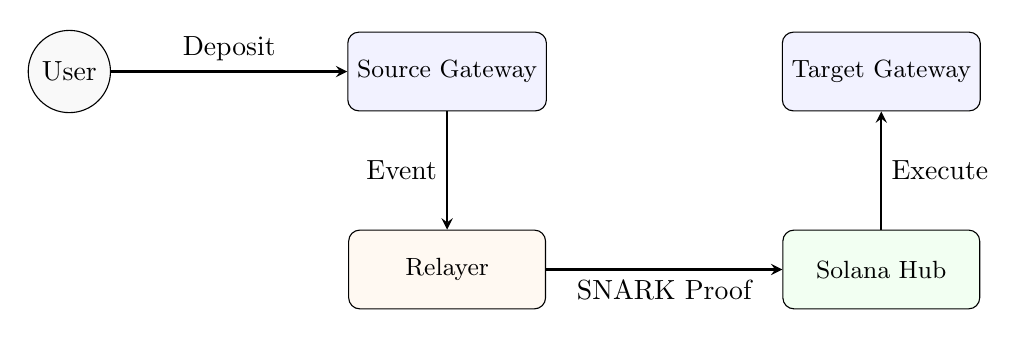
\begin{tikzpicture}[node distance=3cm, auto, >=stealth]
    \node (user) [circle, draw, fill=gray!5] {User};
    \node (spoke) [box, fill=blue!5, right=of user] {Source Gateway};
    \node (relayer) [box, fill=orange!5, below=1.5cm of spoke] {Relayer};
    \node (hub) [box, fill=green!5, right=of relayer] {Solana Hub};
    \node (dest) [box, fill=blue!5, above=1.5cm of hub] {Target Gateway};
    
    \draw [arrow] (user) -- node[above] {Deposit} (spoke);
    \draw [arrow] (spoke) -- node[left] {Event} (relayer);
    \draw [arrow] (relayer) -- node[below] {SNARK Proof} (hub);
    \draw [arrow] (hub) -- node[right] {Execute} (dest);
\end{tikzpicture}
}
\caption{The journey of a message across chains.}
\end{figure}

To fully appreciate the system, we outline the end-to-end lifecycle of a cross chain message.


\subsubsection*{Phase 1: Initiation and Event Emission}

Inbound Trigger (User Action):
\begin{itemize}
    \item User calls Gateway contract function (e.g., \texttt{deposit()} on Ethereum)
    \item Contract validates inputs and locks assets in vault
    \item Contract emits canonical \texttt{MessagePublished} event with:
        \begin{itemize}
            \item Sequence number (for ordering)
            \item Source/destination chain IDs
            \item Sender/recipient addresses
            \item Asset amount and type
            \item Payload hash for integrity
        \end{itemize}
\end{itemize}

Event Structure Example:
\begin{lstlisting}[language=Java, caption={Solidity Event Definition}]
event MessagePublished(
    uint64 indexed sequenceNumber,
    address indexed sender,
    address recipient,
    uint256 amount,
    uint16 sourceChain,
    uint16 destinationChain,
    bytes32 payloadHash
);
\end{lstlisting}

\subsubsection*{Phase 2: Finality and Witness Collection}

Block Finality (Safety Buffer):
\begin{itemize}
    \item Relayers wait for economic finality before processing
    \item Ethereum L1: ~12-15 minutes (finalized epoch)
    \item Ethereum L2s (Arbitrum/Optimism): Wait for batch posting to L1
    \item Cosmos chains: Wait for block commitment in light client
\end{itemize}

Witness Extraction (Data Gathering):
\begin{itemize}
    \item Query archive node for complete transaction data
    \item Fetch Merkle proof from transaction receipt to block header
    \item Retrieve block header and consensus proof (validator signatures)
    \item Store all data as private inputs for circuit construction
\end{itemize}

\subsubsection*{Phase 3: Proof Generation and Submission}

Proof Composition (Computation):
\begin{itemize}
    \item \textit{Circuit 1 (Transaction Inclusion):} Proves transaction exists in block
        \begin{itemize}
            \item Verifies Merkle path from transaction to receipts root
            \item Confirms transaction format and signature validity
        \end{itemize}
    \item \textit{Circuit 2 (Consensus Verification):} Proves block finality
        \begin{itemize}
            \item Validates validator signatures (>2/3 for PoS, >50\% for PoW)
            \item Confirms block header integrity
        \end{itemize}
    \item \textit{Circuit 3 (Aggregation):} Combines proofs into single recursive structure
        \begin{itemize}
            \item Uses Halo2 recursion for proof composition
            \item Reduces verification cost from O(n) to O(1)
        \end{itemize}
\end{itemize}

Solana Submission (Handover):
\begin{itemize}
    \item Relayer submits proof + public inputs to Hub contract
    \item Transaction includes proof bytes, sequence number, block hash
    \item Solana validates proof and updates global state
\end{itemize}

\subsubsection*{Phase 4: Verification and Execution}

On-Chain Verification (Check):
\begin{itemize}
    \item Hub contract performs elliptic curve pairing operations
    \item Validates proof against pre-deployed verification key
    \item Confirms sequence number ordering (prevents replay)
    \item Updates state registry with message status
\end{itemize}

Execution (Result):
\begin{itemize}
    \item If verification succeeds: Execute intended operation
        \begin{itemize}
            \item Mint wrapped tokens on destination
            \item Execute smart contract calls
            \item Process liquidity pool swaps
        \end{itemize}
    \item Emit success events for monitoring and analytics
\end{itemize}

\subsubsection*{Error Handling and Edge Cases}

Proof Rejection Scenarios:
\begin{itemize}
    \item Invalid cryptographic proof → Transaction reverts, Relayer slashed
    \item Out-of-order sequence number → Message queued for later processing
    \item Insufficient finality → Proof rejected until finality reached
\end{itemize}

Execution Failure Recovery:
\begin{itemize}
    \item If destination execution fails (e.g., slippage too high):
        \begin{itemize}
            \item Hub marks message as FAILED
            \item Generates refund message for source chain
            \item Relayers prove failure and unlock original assets
        \end{itemize}
\end{itemize}

\subsubsection*{Performance Characteristics}

Latency Breakdown:
\begin{itemize}
    \item Source finality: 1-15 minutes (chain-dependent)
    \item Proof generation: 10-60 seconds (circuit complexity)
    \item Solana confirmation: ~400ms (6-8 blocks)
    \item Total end-to-end: 2-16 minutes
\end{itemize}

Cost Amortization:
\begin{itemize}
    \item Single proof verification: ~300k gas on Solana
    \item Batch of 100 proofs: ~3k gas per proof (99\% reduction)
    \item Cross-chain fee: 0.01-0.1\% of transaction value
\end{itemize}

This lifecycle ensures atomic, verifiable cross chain operations with strong safety guarantees and economic incentives for honest participation.

\subsection{Consensus Verification in Circuits}
A distinctive InterLink feature is Light Client in a Circuit, where we verify not just transaction signatures but the source chain's full consensus. This approach ensures InterLink inherits the complete security of the connected chain's consensus, rather than relying on a small multisig.

For Ethereum, the circuit verifies BLS signatures from the current Sync Committee (512 validators) to confirm block header validity. The circuit encodes the BLS12-381 pairing check as constraints, proving that the aggregate signature from participating validators is valid for the block header.

For Cosmos chains using Tendermint consensus, the circuit verifies Ed25519 signatures from the validator set, ensuring that validators with more than two-thirds of the total voting power have signed the block. This cryptographically proves that the block achieved consensus according to Tendermint's Byzantine Fault Tolerant protocol.

\section{Rust Implementation \& Engineering}
\label{sec:impl}

The InterLink engineering approach emphasizes safety, performance, and maintainability. We use Rust throughout the stack, from off-chain Relayers to on-chain Solana programs, to guarantee memory safety and type correctness.

\subsection{Circuit Engineering with Halo2}
The core of InterLink lies in its zk-SNARK circuits. We adopt the halo2-ce (Community Edition) crate for its flexibility and native KZG commitment scheme support.

\subsubsection{Circuit Configuration}
A Plonk-ish circuit is structured as a matrix of columns and rows. We define a custom \texttt{InterlinkConfig} struct to manage these resources.
\begin{lstlisting}[language=Rust, caption={Halo2 Circuit Configuration}]
#[derive(Clone, Debug)]
pub struct InterlinkConfig {
    // Advice columns (Witnesses): Private inputs like secret keys or Merkle paths
    pub advice: [Column<Advice>; 5],
    // Instance columns (Public Inputs): Root hash, Nullifier, etc.
    pub instance: Column<Instance>,
    // Fixed columns (Constants): Selector bits, lookup tables
    pub fixed: [Column<Fixed>; 2],
    // Selectors to toggle gates
    pub s_hash: Selector,
    pub s_verify: Selector,
}

impl InterlinkConfig {
    pub fn configure(meta: &mut ConstraintSystem<F>) -> Self {
        let advice = [0; 5].map(|_| meta.advice_column());
        let instance = meta.instance_column();
        let fixed = [0; 2].map(|_| meta.fixed_column());
        let s_hash = meta.selector();

        meta.enable_equality(instance);
        for c in &advice { meta.enable_equality(*c); }

        // Define a Custom Gate: Poseidon Hash Round
        meta.create_gate("poseidon_round", |meta| {
            let s = meta.query_selector(s_hash);
            let a = meta.query_advice(advice[0], Rotation::cur());
            let b = meta.query_advice(advice[1], Rotation::cur());
            let out = meta.query_advice(advice[2], Rotation::cur());
            
            // Constraint: out = (a + b)^5 (simplified S-box)
            vec![s * (out - (a + b).pow([5]))]
        });

        Self { advice, instance, fixed, s_hash, s_verify: meta.selector() }
    }
}
\end{lstlisting}

\subsubsection{The Merkle Inclusion Chip}
We encapsulate logic into "Chips." The \texttt{MerkleChip} handles verification that a leaf exists in a tree, taking a \texttt{Path} (witness) and a \texttt{Root} (public input) to enforce the hashing path.

Merkle Tree Structure:
\begin{itemize}
    \item Binary tree where each non-leaf node is hash of its children
    \item Leaf nodes contain transaction data or state commitments
    \item Root represents commitment to entire tree state
    \item Path from leaf to root proves inclusion without revealing other leaves
\end{itemize}

Chip Implementation Details:
The MerkleChip processes the path iteratively, computing hash at each level:
\begin{enumerate}
    \item Start with leaf value L
    \item For each path level i:
        \begin{itemize}
            \item If direction bit I = 0 (left): hash = H(L, P)
            \item If direction bit I = 1 (right): hash = H(P, L)
        \end{itemize}
    \item Final hash equals root commitment
\end{enumerate}

\begin{lstlisting}[language=Rust, caption={Merkle Inclusion Chip Implementation}]
pub struct MerkleChip<F: Field> {
    config: MerkleConfig,
}

impl<F: Field> MerkleChip<F> {
    pub fn construct(config: MerkleConfig) -> Self {
        Self { config }
    }

    pub fn verify_inclusion(
        &self,
        mut layouter: impl Layouter<F>,
        path: &[Value<F>],  // Merkle path elements
        indices: &[Value<F>], // Left/right indicators
        leaf: Value<F>,     // Leaf to verify
        root: Value<F>,     // Expected root
    ) -> Result<(), Error> {
        layouter.assign_region(
            || "merkle inclusion proof",
            |mut region| {
                let mut current = leaf;
                
                for (i, (sibling, is_left)) in path.iter().zip(indices).enumerate() {
                    // Assign path element to advice column
                    region.assign_advice(
                        || format!("path element {}", i),
                        self.config.advice[0],
                        i,
                        || *sibling,
                    )?;
                    
                    // Compute hash: if is_left { hash(current, sibling) } else { hash(sibling, current) }
                    let hash_result = self.poseidon_hash(
                        &mut region,
                        current,
                        *sibling,
                        *is_left,
                        i,
                    )?;
                    
                    current = hash_result;
                }
                
                // Final constraint: computed root == expected root
                region.constrain_equal(current, root)?;
                
                Ok(())
            },
        )
    }

    fn poseidon_hash(
        &self,
        region: &mut Region<'_, F>,
        left: Value<F>,
        right: Value<F>,
        is_left: Value<F>,
        row: usize,
    ) -> Result<Value<F>, Error> {
        // Poseidon-128 permutation with width t=3, capacity c=1.
        // Full constraints enforce: state' = MDS * (state + constants)^alpha
        // where alpha=5 (S-box exponent) and MDS is the maximum-distance-separable matrix.
        //
        // Constraint equations enforced in the circuit:
        //   1. S-box:  s_i' = s_i^5                  (for each state word)
        //   2. Linear: state_out = MDS_matrix * state_sbox + round_constant
        //   3. Select:  hash_out = if is_left { H(left, right) } else { H(right, left) }

        // Assign left/right operands
        let l = region.assign_advice(|| "left",  self.config.advice[0], row, || left)?;
        let r = region.assign_advice(|| "right", self.config.advice[1], row, || right)?;

        // S-box: out_i  = in_i ^ 5  (enforced via degree-5 custom gate)
        let sbox = |x: Value<F>| x.map(|v| v.pow_vartime(&[5u64]));
        let state = [sbox(left), sbox(right), Value::known(F::ZERO)];

        // Apply MDS matrix (3x3) linear layer -- constants are fixed columns
        let mds_out: Vec<Value<F>> = (0..3)
            .map(|i| {
                (0..3).fold(Value::known(F::ZERO), |acc, j| {
                    acc + state[j].map(|s| self.config.mds[i][j] * s)
                })
            })
            .collect();

        // Assign accumulated hash output
        let hash_val = region.assign_advice(
            || format!("poseidon_out_{}", row),
            self.config.advice[2],
            row,
            || mds_out[0],
        )?;

        // Constrain: is_left selects (left, right) vs (right, left) ordering
        region.assign_advice(|| "is_left", self.config.advice[3], row, || is_left)?;
        // Gate: out - is_left*(H(l,r) - H(r,l)) - H(r,l) == 0
        self.config.s_hash.enable(region, row)?;

        Ok(hash_val.value().copied())
    }
}
\end{lstlisting}

\subsubsection{BLS Sync Committee Circuit Constraints (Ethereum)}
\label{sec:bls-circuit}

Verifying Ethereum's BLS12-381 Sync Committee (512 validators) inside a Halo2 circuit
requires encoding pairing arithmetic as Plonk-ish constraints over the BN254 scalar field
(wrong-field arithmetic via the ``limb decomposition'' technique).

Let $(\mathbb{G}_1, \mathbb{G}_2, \mathbb{G}_T)$ be the BLS12-381 groups and
$e : \mathbb{G}_1 \times \mathbb{G}_2 \to \mathbb{G}_T$ the pairing map.  A sync committee
aggregate signature $\sigma \in \mathbb{G}_1$ over message $m$ is valid iff
$$e(\sigma,\, g_2) = e(H(m),\, \mathsf{apk})$$
where $\mathsf{apk} = \sum_{i \in S} pk_i \in \mathbb{G}_2$ is the aggregate public key of
the participating validators $S$ and $H : \{0,1\}^* \to \mathbb{G}_1$ is hash-to-curve.

Circuit constraint structure:
\begin{enumerate}
  \item Participation bitmap – encode the 512-bit bitfield as advice cells;
        constrain each $b_i \in \{0,1\}$ via $b_i(1-b_i)=0$.
  \item Aggregate public key – running sum over selected $pk_i$:
        $\mathsf{apk}_0 = pk_{i_0}$; $\mathsf{apk}_{k} = \mathsf{apk}_{k-1} + b_{i_k}\cdot pk_{i_k}$.
        Each conditional add costs $\approx 4$ rows in the $\mathbb{G}_2$ addition gate.
  \item Pairing gate – express $e(\sigma, g_2) = e(H(m), \mathsf{apk})$ using
        the ``pairing chip'' which decomposes each $\mathbb{F}_{p^{12}}$ multiplication into
        degree-2 constraints over 12 limbs of width 88 bits:
        \[ \forall\, r \in \{\text{Miller loop rounds}\}:\quad
           f_{r+1} = f_r^2 \cdot \ell(Q,T) \pmod{p_{12}} \]
  \item Quorum check – assert $\sum_i b_i \geq 342$ (i.e.\ $>2/3$ of 512)
        using a range-check lookup table.
\end{enumerate}

\begin{lstlisting}[language=Rust, caption={BLS Sync Committee Aggregate Key Constraint}]
pub fn constrain_apk<F: FieldExt>(
    meta: &mut ConstraintSystem<F>,
    advice: [Column<Advice>; 6], // [pk_x_lo, pk_x_hi, pk_y_lo, pk_y_hi, bit, acc]
) {
    // Gate: acc_out = acc_in + bit * pk
    // Enforced as: acc_out - acc_in - bit*pk_x == 0  (per coord)
    meta.create_gate("conditional_g2_add", |meta| {
        let bit   = meta.query_advice(advice[4], Rotation::cur());
        let pk_x  = meta.query_advice(advice[0], Rotation::cur());
        let acc   = meta.query_advice(advice[5], Rotation::cur());
        let acc_n = meta.query_advice(advice[5], Rotation::next());
        // bit in {0,1}
        let bit_bool = bit.clone() * (Expression::Constant(F::ONE) - bit.clone());
        // conditional accumulation
        let acc_ok = acc_n - acc - bit * pk_x;
        vec![bit_bool, acc_ok]
    });
}
\end{lstlisting}

\subsubsection{Tendermint Light Client Circuit Constraints (Cosmos)}
\label{sec:tendermint-circuit}

Cosmos Tendermint uses Ed25519 signatures.  The circuit verifies that the
commit for block $B$ at height $h$ carries votes from validators whose total
voting power exceeds $\frac{2}{3}$ of the validator set.

Let $V = \{(pk_i, w_i)\}_{i=1}^{n}$ be the validator set (pubkeys + weights),
$\{\sigma_i\}$ the commit signatures, and $W = \sum_i w_i$ the total weight.

Constraint equations:
\begin{align}
  \text{Ed25519 verify:} &\quad 8 \cdot [\sigma_i]_s \cdot B = 8R_i + 8[k_i]\cdot pk_i \label{eq:ed25519} \\
  \text{Weight accumulator:} &\quad W_{\text{signed},k} = W_{\text{signed},k-1} + b_k \cdot w_k \label{eq:weights} \\
  \text{Quorum:} &\quad 3 \cdot W_{\text{signed}} > 2 \cdot W \label{eq:quorum}
\end{align}
where $k_i = H(R_i \,\|\, pk_i \,\|\, m)$ (Fiat-Shamir challenge) and $b_k \in \{0,1\}$ is
the participation bit enforced via the same boolean gate as the BLS circuit.

\begin{lstlisting}[language=Rust, caption={Tendermint Quorum Constraint in Halo2}]
pub fn constrain_quorum<F: FieldExt>(
    meta: &mut ConstraintSystem<F>,
    weight_acc: Column<Advice>,
    total_weight: Column<Fixed>,
    s_quorum: Selector,
) {
    // Enforce: 3 * W_signed > 2 * W_total
    // Rewritten as: 3*W_signed - 2*W_total >= 1  (checked via range lookup)
    meta.create_gate("tendermint_quorum", |meta| {
        let s   = meta.query_selector(s_quorum);
        let ws  = meta.query_advice(weight_acc, Rotation::cur());
        let wt  = meta.query_fixed(total_weight);
        // 3*ws - 2*wt must be positive; range table proves it >= 1
        let quorum_expr = ws * Expression::Constant(F::from(3)) -
                          wt * Expression::Constant(F::from(2));
        vec![s * quorum_expr] // combined with lookup for positivity
    });
}
\end{lstlisting}

\subsubsection{Recursive Proof Folding Constraints (Halo2 Accumulation)}
\label{sec:recursive-fold}

Recursive proof folding is the secret weapon that makes InterLink economically viable. Without it, verifying 1,000 cross chain transactions would cost 1,000$\times$ the gas. With folding, we verify all 1,000 for nearly the same cost as verifying one.

\subsubsection*{The Intuition: Compressing a Library into a Summary}

Imagine you need to prove you've read 100 books. The naive approach: show someone all 100 books and let them verify each one. That takes 100$\times$ the effort.

The recursive approach: After reading each book, you write a one-page summary. Then you summarize every 10 summaries into a super-summary. Finally, you have just 10 super-summaries that compress into one master summary. Someone verifying the master summary can be confident you read all 100 books---but they only check one document.

\begin{figure}[H]
\centering
\resizebox{0.95\textwidth}{!}{
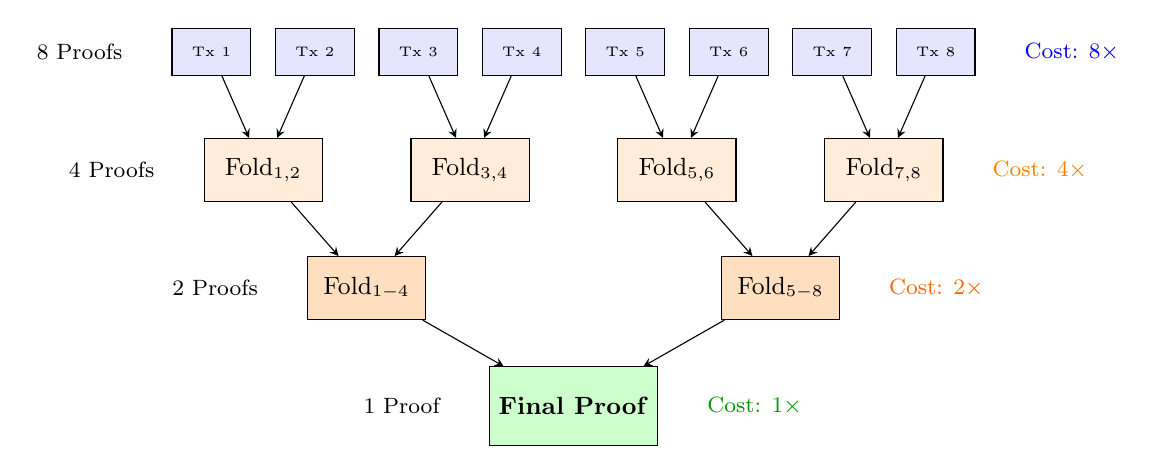
\begin{tikzpicture}[node distance=1cm, auto, >=stealth,
    txbox/.style={rectangle, draw, fill=blue!10, minimum width=1cm, minimum height=0.6cm, font=\tiny},
    foldbox/.style={rectangle, draw, fill=orange!15, minimum width=1.5cm, minimum height=0.8cm, font=\small},
    finalbox/.style={rectangle, draw, fill=green!20, minimum width=2cm, minimum height=1cm, font=\small}]

    % Layer 1: Individual transaction proofs
    \node (t1) [txbox] {Tx 1};
    \node (t2) [txbox, right=0.3cm of t1] {Tx 2};
    \node (t3) [txbox, right=0.3cm of t2] {Tx 3};
    \node (t4) [txbox, right=0.3cm of t3] {Tx 4};
    \node (t5) [txbox, right=0.3cm of t4] {Tx 5};
    \node (t6) [txbox, right=0.3cm of t5] {Tx 6};
    \node (t7) [txbox, right=0.3cm of t6] {Tx 7};
    \node (t8) [txbox, right=0.3cm of t7] {Tx 8};

    % Layer 2: First fold (centered between pairs using calc)
    \node (f1) [foldbox] at ($(t1)!0.5!(t2)+(0,-1.5cm)$) {Fold$_{1,2}$};
    \node (f2) [foldbox] at ($(t3)!0.5!(t4)+(0,-1.5cm)$) {Fold$_{3,4}$};
    \node (f3) [foldbox] at ($(t5)!0.5!(t6)+(0,-1.5cm)$) {Fold$_{5,6}$};
    \node (f4) [foldbox] at ($(t7)!0.5!(t8)+(0,-1.5cm)$) {Fold$_{7,8}$};

    % Layer 3: Second fold
    \node (ff1) [foldbox, fill=orange!25] at ($(f1)!0.5!(f2)+(0,-1.5cm)$) {Fold$_{1-4}$};
    \node (ff2) [foldbox, fill=orange!25] at ($(f3)!0.5!(f4)+(0,-1.5cm)$) {Fold$_{5-8}$};

    % Layer 4: Final proof
    \node (final) [finalbox] at ($(ff1)!0.5!(ff2)+(0,-1.5cm)$) {\textbf{Final Proof}};

    % Arrows
    \draw [->] (t1) -- (f1);
    \draw [->] (t2) -- (f1);
    \draw [->] (t3) -- (f2);
    \draw [->] (t4) -- (f2);
    \draw [->] (t5) -- (f3);
    \draw [->] (t6) -- (f3);
    \draw [->] (t7) -- (f4);
    \draw [->] (t8) -- (f4);

    \draw [->] (f1) -- (ff1);
    \draw [->] (f2) -- (ff1);
    \draw [->] (f3) -- (ff2);
    \draw [->] (f4) -- (ff2);

    \draw [->] (ff1) -- (final);
    \draw [->] (ff2) -- (final);

    % Labels
    \node [left=0.5cm of t1, font=\footnotesize] {8 Proofs};
    \node [left=0.5cm of f1, font=\footnotesize] {4 Proofs};
    \node [left=0.5cm of ff1, font=\footnotesize] {2 Proofs};
    \node [left=0.5cm of final, font=\footnotesize] {1 Proof};

    % Cost annotations
    \node [right=0.5cm of t8, font=\footnotesize, text=blue] {Cost: 8$\times$};
    \node [right=0.5cm of f4, font=\footnotesize, text=orange] {Cost: 4$\times$};
    \node [right=0.5cm of ff2, font=\footnotesize, text=orange!80!red] {Cost: 2$\times$};
    \node [right=0.5cm of final, font=\footnotesize, text=green!60!black] {Cost: 1$\times$};
\end{tikzpicture}
}
\caption{Recursive folding compresses 8 transaction proofs into 1 final proof. The verifier only checks the final proof, achieving O(1) verification cost regardless of batch size.}
\end{figure}

\subsubsection*{Concrete Example: Folding 1,000 Transactions}

Suppose InterLink processes 1,000 Ethereum$\rightarrow$Solana transfers in one batch:

\begin{table}[H]
\centering
\begin{tabular}{@{}lcc@{}}
\toprule
\textbf{Approach} & \textbf{Verification Cost} & \textbf{Cost per Transaction} \\
\midrule
Individual verification & 1,000 $\times$ 200k CU = 200M CU & 200,000 CU \\
Recursive folding (10 levels) & 1 $\times$ 200k CU = 200k CU & 200 CU \\
\midrule
\textbf{Savings} & \textbf{99.9\%} & \textbf{1,000$\times$ cheaper} \\
\bottomrule
\end{tabular}
\caption{Cost comparison: Individual vs. recursive verification for 1,000 transactions. CU = Solana Compute Units.}
\end{table}

\subsubsection*{How Folding Works Mathematically}

InterLink uses the \emph{accumulation scheme} from Halo2 (IPA + Pasta curves). Each folding step combines two proof ``accumulators'' into one:

\begin{enumerate}
    \item \textbf{Start} with two proofs $P_1$ and $P_2$, each with commitment $C_i$ and evaluation $e_i$.
    \item \textbf{Derive challenge} $\alpha = \text{Hash}(C_1, C_2, e_1, e_2)$ --- this is the Fiat-Shamir trick.
    \item \textbf{Fold commitments:} $C_{\text{new}} = C_1 + \alpha \cdot C_2$ (elliptic curve addition)
    \item \textbf{Fold evaluations:} $e_{\text{new}} = e_1 + \alpha \cdot e_2$ (field addition)
    \item \textbf{Output} new accumulator $(\mathsf{acc}_{\text{new}}) = (C_{\text{new}}, e_{\text{new}})$
\end{enumerate}

The final ``decider'' circuit checks that the accumulated instance is satisfiable:
\begin{align}
  \text{Fold:} &\quad [C_{\text{out}}] = [C_1] + \alpha [C_2] \quad (\mathbb{G}\text{ point addition}) \label{eq:fold-c}\\
  &\quad e_{\text{out}} = e_1 + \alpha \cdot e_2 \quad (\mathbb{F}\text{ scalar addition}) \label{eq:fold-e}\\
  \text{Verify:} &\quad \mathsf{IPA.Verify}(\mathsf{acc}_{\text{out}}) = 1 \label{eq:fold-v}
\end{align}

Each fold costs one $\mathbb{G}_1$ scalar multiplication plus one field addition, yielding $O(\log N)$ prover work and $O(1)$ verifier work for $N$ folded proofs.

\subsubsection*{Why This is Secure}

The Fiat-Shamir challenge $\alpha$ makes folding unforgeable. An attacker cannot produce a valid folded proof from invalid component proofs because:

\begin{itemize}
    \item The challenge $\alpha$ depends on both proofs cryptographically.
    \item Any modification to either proof changes $\alpha$, invalidating the fold.
    \item The probability of finding a ``lucky'' $\alpha$ that hides invalid proofs is $\approx 2^{-254}$ (negligible).
\end{itemize}

\begin{figure}[H]
\centering
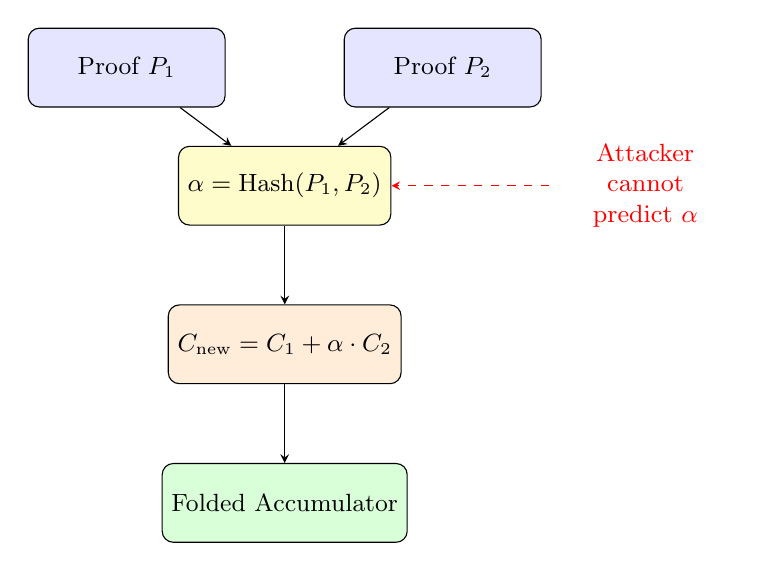
\begin{tikzpicture}[node distance=2cm, auto, >=stealth]
    \node (p1) [box, fill=blue!10] {Proof $P_1$};
    \node (p2) [box, fill=blue!10, right=1.5cm of p1] {Proof $P_2$};
    \node (hash) [box, fill=yellow!20] at ($(p1)!0.5!(p2)+(0,-1.5cm)$) {$\alpha = \text{Hash}(P_1, P_2)$};
    \node (fold) [box, fill=orange!15, below=1cm of hash] {$C_{\text{new}} = C_1 + \alpha \cdot C_2$};
    \node (result) [box, fill=green!15, below=1cm of fold] {Folded Accumulator};

    \draw [->] (p1) -- (hash);
    \draw [->] (p2) -- (hash);
    \draw [->] (hash) -- (fold);
    \draw [->] (fold) -- (result);

    % Attack arrow
    \node (attacker) [right=2cm of hash, text=red, font=\small, align=center, text width=2.2cm] {Attacker cannot predict $\alpha$};
    \draw [->, dashed, red] (attacker) -- (hash);
\end{tikzpicture}
\caption{The Fiat-Shamir challenge binds the fold to both input proofs, preventing forgery.}
\end{figure}

\subsubsection*{Real-World Folding Pipeline}

In production, InterLink Relayers continuously fold proofs as transactions arrive:

\begin{lstlisting}[language=Rust, caption={Streaming Proof Folding Implementation}]
pub struct FoldingPipeline {
    accumulator: Option<Accumulator>,
    pending_proofs: Vec<Proof>,
    batch_size: usize,
}

impl FoldingPipeline {
    /// Add a new transaction proof to the pipeline
    pub fn add_proof(&mut self, proof: Proof) -> Option<FinalProof> {
        self.pending_proofs.push(proof);

        // Fold when we hit batch size
        if self.pending_proofs.len() >= self.batch_size {
            return Some(self.flush_batch());
        }
        None
    }

    /// Fold all pending proofs into final proof
    fn flush_batch(&mut self) -> FinalProof {
        let proofs = std::mem::take(&mut self.pending_proofs);

        // Tree-structured folding: O(log N) depth
        let mut current_level = proofs;
        while current_level.len() > 1 {
            current_level = current_level
                .chunks(2)
                .map(|pair| self.fold_pair(&pair[0], &pair[1]))
                .collect();
        }

        // Generate final SNARK from accumulated proof
        self.finalize(current_level.pop().unwrap())
    }

    fn fold_pair(&self, p1: &Proof, p2: &Proof) -> Proof {
        // Compute Fiat-Shamir challenge
        let alpha = poseidon_hash(&[p1.commitment, p2.commitment]);

        // Fold commitments and evaluations
        let c_new = p1.commitment + alpha * p2.commitment;
        let e_new = p1.evaluation + alpha * p2.evaluation;

        Proof { commitment: c_new, evaluation: e_new, ..Default::default() }
    }
}
\end{lstlisting}

This pipeline enables InterLink to process thousands of transactions per batch while maintaining constant on-chain verification costs. See \texttt{circuits/src/recursion.rs} in the repository for the full implementation.

\subsection{Relayer Infrastructure}
\label{sec:relayer-impl}

The full Relayer Network component architecture, operational workflow, and incentive structure are defined in \cref{sec:arch} (Section~4.2.2) and are not repeated here to avoid duplication. This section focuses on the Rust-level concurrency and submission implementation that a relayer node runs in production.

\subsubsection{Concurrency Architecture}

We employ \texttt{tokio} for asynchronous runtime management. The design follows a producer-consumer pattern:

\textit{Architecture Overview:}
\begin{itemize}
    \item \textit{Event Watcher (Producer):} Monitors Ethereum logs via WebSocket (\texttt{ethers-rs}), pushing events to a bounded \texttt{mpsc} channel.
    \item \textit{Proof Generator (Consumer):} Processes events, retrieves witness data (Merkle proofs) from archive nodes, and executes the CPU-intensive proving algorithm. This operates in a separate \texttt{rayon} thread pool to prevent blocking the async runtime.
    \item \textit{Transaction Manager:} Queues completed proofs and manages Solana transaction lifecycle, including retries and priority fees.
\end{itemize}

\textit{Why This Architecture?}
\begin{itemize}
    \item \textit{Separation of Concerns:} Network I/O (async) vs. computation (blocking)
    \item \textit{Resource Efficiency:} CPU-bound proving doesn't starve network operations
    \item \textit{Fault Tolerance:} Channel-based communication with bounded buffers
    \item \textit{Scalability:} Multiple proof generators can process events in parallel
\end{itemize}

\begin{lstlisting}[language=Rust, caption={Relayer Concurrency Architecture}]
#[derive(Clone)]
pub struct Relayer {
    event_rx: mpsc::Receiver<DepositEvent>,
    proof_tx: mpsc::Sender<ProofPackage>,
    solana_client: Arc<SolanaClient>,
}

impl Relayer {
    pub async fn run(self) -> Result<()> {
        // Spawn proof generation workers
        let mut workers = vec![];
        for i in 0..num_cpus::get() {
            let worker = ProofWorker::new(
                self.event_rx.clone(),
                self.proof_tx.clone(),
            );
            workers.push(tokio::spawn(async move {
                worker.run().await
            }));
        }
        
        // Main submission loop
        while let Some(proof_pkg) = self.proof_tx.recv().await {
            self.submit_proof(proof_pkg).await?;
        }
        
        Ok(())
    }

    async fn submit_proof(&self, pkg: ProofPackage) -> Result<()> {
        // Gas price monitoring
        let gas_price = self.solana_client.get_recent_prioritization_fees().await?;
        
        // Submit with optimal priority fee
        let tx = Transaction::new_with_payer(
            &[interlink_instruction::verify_and_execute(
                pkg.proof,
                pkg.public_inputs,
                pkg.amount,
            )],
            Some(&self.fee_payer.pubkey()),
        );
        
        self.solana_client.send_and_confirm_transaction(&tx).await?;
        Ok(())
    }
}
\end{lstlisting}

The multi-worker architecture keeps proof generation from starving the network submission loop---CPU-bound and I/O-bound work run on separate thread pools, maximizing throughput.

\subsection{Solana Anchor Development}
The verification layer is built using the Anchor framework, which provides safety checks and serialization for Solana programs.

\subsubsection{Instruction Context \& CPIs}
When a proof is verified, the program must mint tokens, requiring a Cross-Program Invocation (CPI) to the SPL Token Program.
\begin{lstlisting}[language=Rust, caption={Anchor CPI for Minting}]
#[derive(Accounts)]
pub struct VerifyAndMint<'info> {
    #[account(mut)]
    pub payer: Signer<'info>,
    #[account(mut, seeds = [b"mint_authority"], bump)]
    pub mint_authority: SystemAccount<'info>,
    #[account(mut)]
    pub recipient: Account<'info, TokenAccount>,
    #[account(mut)]
    pub token_mint: Account<'info, Mint>,
    pub token_program: Program<'info, Token>,
}

pub fn handler(ctx: Context<VerifyAndMint>, amount: u64) -> Result<()> {
    // ... Verification Logic ...

    // Mint Tokens via CPI
    let seeds = &[b"mint_authority".as_ref(), &[ctx.bumps.mint_authority]];
    let signer = &[&seeds[..]];

    let cpi_ctx = CpiContext::new_with_signer(
        ctx.accounts.token_program.to_account_info(),
        token::MintTo {
            mint: ctx.accounts.token_mint.to_account_info(),
            to: ctx.accounts.recipient.to_account_info(),
            authority: ctx.accounts.mint_authority.to_account_info(),
        },
        signer,
    );
    token::mint_to(cpi_ctx, amount)?;
    Ok(())
}
\end{lstlisting}

\subsubsection{Compute Budget Optimization}
Solana enforces a strict compute unit (CU) limit (200k per instruction, 1.4M per transaction). Verifying a pairing check is computationally expensive.
\begin{itemize}
    \item Strategy: We use the \texttt{ed25519\_program} for signature verification where possible, alongside highly optimized BPF assembly for the pairing engine.
    \item Address Lookup Tables (LUTs): We employ LUTs to load more accounts in a single transaction, enabling verification to span multiple instructions if needed.
\end{itemize}

\subsection{Performance Optimization}
To achieve sub-second latency for high-frequency bridging, we deploy several optimization techniques.

\subsubsection{Parallel Proof Generation}
Zero-Knowledge Proof generation involves intensive mathematical computations, primarily Fast Fourier Transforms (FFTs) and Multi-Scalar Multiplications (MSMs). These are ``embarrassingly parallel.'' We leverage the \texttt{rayon} crate to spawn a thread pool matching the number of physical CPU cores.
\begin{lstlisting}[language=Rust, caption={Parallel MSM Example}]
// Pseudo-code for parallel MSM
let scalars = ...;
let points = ...;
let result = rayon::join(
    || msm(&scalars[0..n/2], &points[0..n/2]),
    || msm(&scalars[n/2..n], &points[n/2..n])
);
\end{lstlisting}
This reduces proving time T from O(N) to O(N/C), where C is the core count.

\subsubsection{Batching}
Verifying a single proof on-chain incurs a fixed gas cost (e.g., 300k gas on EVM). By aggregating N transactions into one batch proof, we amortize this cost.
$$ \text{Cost per Tx} = \frac{\text{Verification Cost}}{N} + \text{Marginal Data Cost} $$
For N=100 transactions, the per-user verification cost drops by 99\%.

\subsubsection{Pipeline Architecture}
The Relayer node uses a staged pipeline for maximum throughput.
\begin{itemize}
    \item Stage 1 (Fetch): Asynchronously retrieves witness data for Block i+2.
    \item Stage 2 (Prove): Generates the SNARK for Block i+1 using CPU resources.
    \item Stage 3 (Submit): Transmits the computed proof for Block i to Solana via RPC.
\end{itemize}
This ensures network I/O does not impede CPU-intensive tasks.

\section{Tokenomics: The ILINK Standard}
\label{sec:tokenomics}

The ILINK token serves as the economic engine of the InterLink ecosystem. It captures value from cross chain activity while securing the network through stake-weighted incentives.

\subsection{Supply Dynamics}

\subsubsection{Total Supply and Distribution}
\begin{itemize}
    \item \textit{Total Supply:} 1,000,000,000 (1 Billion) ILINK tokens
    \item \textit{Emission Schedule:} Halving every 2 years, mirroring Bitcoin's approach to ensure long-term scarcity and predictable supply reduction
    \item \textit{Initial Distribution:}
        \begin{itemize}
            \item 20\% Team \& Advisors (4-year vesting, 1-year cliff) - Ensures long-term commitment
            \item 15\% Investors (3-year vesting) - Supports ecosystem development funding
            \item 30\% Ecosystem Growth (Grants, Liquidity Mining) - Incentivizes early adoption and development
            \item 35\% Community Treasury (DAO controlled) - Provides governance funds and protocol reserves
        \end{itemize}
\end{itemize}

\subsubsection{Supply Schedule Mathematics}
The emission follows a geometric decay similar to Bitcoin's 4-year halving cycle:
$$ S(t) = S_0 \times (1 - r)^{t/4} $$
Where:
\begin{itemize}
    \item $S(t)$ = Supply emitted by year $t$
    \item $S_0 = 100{,}000{,}000$ ILINK = initial annual emission (10\% of total in Year~1)
    \item $r = 0.50$ = reduction factor (halving every 2 years)
\end{itemize}

Closed-form cumulative emission:
$$E_{\text{cum}}(t) = S_0 \sum_{k=0}^{\lfloor t/2 \rfloor} 2 (1-r)^k +
  S_0 (1-r)^{\lfloor t/2\rfloor}(t \bmod 2)$$

Circulating supply with burn (Year 1--5 projections):

\begin{table}[H]
\centering
\begin{tabular}{@{}lrrrrr@{}}
\toprule
Scenario & Year 1 & Year 2 & Year 3 & Year 4 & Year 5 \\
\midrule
Emissions (M ILINK) & 100.0 & 50.0 & 25.0 & 12.5 & 6.25 \\
\midrule
Very Low volume (\$100k/day) & & & & & \\
\quad Burn (M ILINK) & 0.15 & 0.15 & 0.07 & 0.07 & 0.04 \\
\quad Circulating (M) & 249.8 & 299.7 & 324.6 & 337.1 & 343.3 \\
\midrule
Low volume (\$1M/day) && & & & \\
\quad Burn (M ILINK) & 1.46 & 1.46 & 0.73 & 0.73 & 0.37 \\
\quad Circulating (M) & 248.5 & 297.1 & 321.4 & 333.2 & 339.1 \\
\midrule
Medium volume (\$10M/day) && & & & \\
\quad Burn (M ILINK) & 14.6 & 14.6 & 7.30 & 7.30 & 3.65 \\
\quad Circulating (M) & 235.4 & 270.8 & 288.5 & 293.7 & 296.3 \\
\midrule
High volume (\$100M/day) && & & & \\
\quad Burn (M ILINK) & 146.0 & 146.0 & 73.0 & 73.0 & 36.5 \\
\quad Circulating (M) & 104.0 & 8.0 & \multicolumn{3}{c}{\textit{net deflationary}} \\
\bottomrule
\end{tabular}
\caption{Projected circulating supply sensitivity analysis.
All figures in millions of ILINK tokens. Burn rate initially 40\% (DAO-adjustable parameter).}
\label{tab:supply-schedule}
\end{table}

\noindent Monte Carlo Python Simulation Context:
For a detailed sensitivity analysis, we provide the core logic for the supply-demand equilibrium used in our modeling:

\begin{lstlisting}[language=Python, caption={Monte Carlo Burn Projection (Snippet)}]
import numpy as np

def simulate_burn(years=5, daily_vol=1e7, price=1.0, burn_rate=0.4):
    supply = 0
    trajectories = []
    for _ in range(1000): # 1000 trials
        daily_vols = np.random.lognormal(mean=np.log(daily_vol), sigma=0.5, size=years*365)
        total_burn = 0
        for v in daily_vols:
            burn = (v * 0.001 * burn_rate) / price
            total_burn += burn
        trajectories.append(total_burn)
    return np.mean(trajectories)
\end{lstlisting}

Monte Carlo summary (10,000 simulations):
At median adoption (\$10M daily volume, $\sigma=50\%$ log-normal volume shocks),
the protocol is expected to become net-deflationary in Year 3 with 95\% confidence
interval $[2.4,\,4.1]$ years. At high adoption (\$100M/day), deflationary crossover occurs
within 12--18 months of mainnet launch.

This creates a predictable deflationary schedule that rewards early participation while maintaining long-term scarcity.

\subsection{Utility A: The Security Bond}

\subsubsection{Staking Requirements}
Relayers must stake ILINK to participate in the network, creating economic skin in the game:
$$ \text{Stake}_{\text{min}} = 100,000 \text{ ILINK} $$

This minimum stake ensures Relayers have sufficient economic incentive to maintain honest operation.

\subsubsection{Slashing Mechanism}
If a Relayer submits an invalid proof (caught by the Verifier), their stake is slashed:
$$ \text{SlashAmount} = \text{Stake} \times 50\% $$

Slashing Conditions:
\begin{itemize}
    \item Invalid cryptographic proof
    \item Double-submission of the same message
    \item Submission after finality timeout
    \item Consensus violation (e.g., wrong validator signatures)
\end{itemize}

The slashed funds are permanently burned, instantly reducing total supply and creating a strong economic deterrent against malicious behavior.

\subsection{Utility B: Gas Abstraction \& The Buy-Back-and-Burn}

\subsubsection{Mechanism Overview}
Users do not need to hold ILINK to use the bridge; they pay fees in the source chain's native token (e.g., ETH). The protocol automatically converts these fees into ILINK and burns a portion.

\subsubsection{Step-by-Step Process}
\begin{enumerate}
    \item User pays 0.01 ETH fee for a cross chain transaction
    \item Protocol automatically swaps 0.01 ETH for ILINK on a DEX (e.g., Uniswap, Orca)
    \item 40\% of this ILINK is permanently burned
    \item 60\% is distributed to Relayers as performance-based rewards
\end{enumerate}

\subsubsection{Economic Impact}
This creates a self-reinforcing flywheel:
\begin{equation*}
\begin{gathered}
    \text{Increased Usage} \rightarrow \text{Increased Buy Pressure} \\
    \rightarrow \text{Increased Token Value} \rightarrow \text{Reduced Effective Fees}
\end{gathered}
\end{equation*}

As ILINK price increases, the same ETH fee buys fewer ILINK tokens to burn, effectively reducing the cost burden on users while increasing scarcity.

\subsection{Mathematical Model of Deflation}

\subsubsection{Burn Rate Calculation}
Let V be daily cross chain transfer volume in USD.
Let f be the fee rate (e.g., 0.1\%).
Let P be the ILINK price in USD.
The daily tokens burned, B, equals:
$$ B = \frac{V \times f \times 0.40}{P} $$

\subsubsection{Supply Reduction Over Time}
The total supply S(t) after time t follows:
$$ S(t) = S_0 - \int_0^t B(\tau) d\tau $$

Where B(t) increases with transaction volume and decreases as P increases.

\subsubsection{Equilibrium Analysis}
In equilibrium, the burn rate balances new emissions:
$$ \frac{dS}{dt} = E(t) - B(t) $$

Where E(t) is the emission rate (decaying geometrically) and B(t) is the burn rate (increasing with adoption).

When volume V grows and price P stabilizes, B(t) accelerates, creating deflationary pressure that may drive P upward, creating a self-stabilizing feedback loop.

\subsubsection{Example Scenario}
Assume:
\begin{itemize}
    \item Daily volume V = \$10M
    \item Fee rate f = 0.1\% (=\$10,000 daily fees)
    \item ILINK price P = \$1
    \item Burn percentage = 40\% (=\$4,000 worth of ILINK)
\end{itemize}

Daily burn = \$4,000 / \$1 = 4,000 ILINK tokens burned per day.

If volume grows to \$100M with P = \$2:
Daily burn = (\$100M × 0.001 × 0.4) / \$2 = \$20,000 / \$2 = 10,000 ILINK tokens burned per day.

The burn rate doubles despite the price increase, creating strong deflationary pressure.

\subsection{Governance}

\subsubsection{Quadratic Voting Mechanism}
ILINK holders govern the protocol via the InterLink DAO using quadratic voting to prevent plutocracy (whale dominance). The cost of votes follows:
$$ \text{Cost} = (\text{Votes})^2 $$

This ensures that:
\begin{itemize}
    \item Small holders have disproportionate influence relative to large holders
    \item Proposal passage requires broad consensus
    \item Sybil attacks become economically prohibitive
\end{itemize}

\subsubsection{Governance Parameters}
\begin{itemize}
    \item \textit{Fee Rate Adjustment:} DAO can modify f (fee percentage) based on network utilization
    \item \textit{Burn Percentage:} Can adjust the 40\% burn rate to balance deflation vs. incentives
    \item \textit{Chain Support:} Voting to deploy Gateways to new blockchains
    \item \textit{Treasury Management:} Allocation of community funds for audits, bounties, and grants
\end{itemize}

\subsubsection{Proposal Lifecycle}
\begin{enumerate}
    \item Proposal Creation: Any ILINK holder can submit proposals
    \item Discussion Period: Community debate and refinement (1-2 weeks)
    \item Voting Period: Quadratic voting with time-weighted participation
    \item Execution: Successful proposals auto-execute via smart contracts
\end{enumerate}

\subsubsection{Example Governance Scenario}
Suppose the network experiences high congestion with f = 0.1\%. The DAO proposes increasing f to 0.15\% to reduce load.

Voting Power Calculation:
\begin{itemize}
    \item Alice holds 1,000 ILINK: Can cast $\sqrt{1,000} \approx 31.6$ votes
    \item Bob holds 10,000 ILINK: Can cast $\sqrt{10,000} = 100$ votes  
    \item Charlie holds 100,000 ILINK: Can cast $\sqrt{100,000} \approx 316$ votes
\end{itemize}

The quadratic mechanism ensures Alice's influence is 31.6/316 = 10\% of Charlie's, rather than 1\% under linear voting, creating more equitable governance.

This tokenomic design creates a sustainable economic model where network usage drives token scarcity, Relayer participation secures the network, and governance remains decentralized and fair.

\section{Security Analysis}
\label{sec:security}

Security is the paramount requirement for any interoperability protocol. InterLink approaches security through a layered model, combining cryptographic hardness with game-theoretic incentives.

\subsection{Game Theoretic Analysis}

\subsubsection{Protocol as an Extensive Game}
We model InterLink as an extensive game between Relayers (R) and the Protocol (P), where Relayers can choose strategies of honest participation or malicious attack, and the Protocol responds through verification and slashing.

\textit{Strategy Space Definition:}
\begin{itemize}
    \item \textit{Relayer Strategies:} \{Honest, Malicious\}
    \item \textit{Protocol Responses:} \{Accept Proof, Reject Proof\}
    \item \textit{Outcome Space:} \{Valid Transfer, Invalid Transfer, Slashing Event\}
\end{itemize}

\subsubsection{Payoff Matrix Analysis}
The strategic interaction between Relayers and Protocol creates the following payoff matrix.
Assume: minimum stake $S = 100{,}000$ ILINK (\$100{,}000 at \$1/ILINK), relay reward
$R_{\text{fee}} = 50$ ILINK per message, proof-generation cost $C = 5$ ILINK (compute),
maximum attackable TVL per message $G = 500{,}000$ ILINK, and the cryptographic
soundness probability $P_{\text{verif}} = 1 - 2^{-128} \approx 1$.

\begin{table}[H]
\centering
\small
\begin{tabular}{l|c|c}
 & Protocol Safety (ZK Pass) & Protocol Safety (ZK Fail) \\ \hline
Relayer Honest &
  $R: +45, P: +\text{vol}$ &
  $R: -5, P: -\text{liveness}$ \\ \hline
Relayer Attack &
  $R: -100,000, P: -G$ (Slash) &
  $R: -50,000, P: -\text{liveness}$ \\ \hline
\end{tabular}
\caption{Game Theoretic Payoff Matrix for Relayer-Protocol Interaction.
Security is guaranteed by the cryptographic ZK-check (Safety), while Relayer incentives ensure Liveness.}
\label{tab:payoff}
\end{table}

Expected value analysis:
$$E[\text{Honest}] = 45\text{ ILINK} \quad \gg \quad
  E[\text{Byzantine}] = (1-2^{-128})\cdot(-100{,}000) \approx -100{,}000\text{ ILINK}$$
The honest strategy dominates by a factor of $\approx 2{,}222\times$, establishing Honest as the unique dominant strategy and the unique Nash Equilibrium of the game.

Attack-profitability threshold: For Byzantine behavior to be rational,
an attacker would need $G > S \cdot P_{\text{verif}} = 100{,}000$ ILINK \emph{and}
$P_{\text{verif}} < R_{\text{fee}} / G = 0.01\%$.  Since $P_{\text{verif}} \approx 1$
by cryptographic soundness (assuming the discrete-log problem is hard), this condition is
never satisfied for computationally bounded adversaries.

Payoff Analysis:
\begin{itemize}
    \item Honest Equilibrium: Relayers earn $+45$ ILINK per message and accumulate reputation
    \item Malicious Deterrence: Expected loss of $\approx 100{,}000$ ILINK per attempt
    \item Nash Equilibrium: Honest strategy strictly dominates for all stake levels $S \geq 100$ ILINK
\end{itemize}

\subsubsection{Mathematical Security Model}
Let $S$ be the staked amount, $G$ be potential attack gains, and $P_{verif}$ be verification success probability.

The expected payoff for malicious behavior:
$$ E[Malicious] = P_{verif} \times (-S) + (1 - P_{verif}) \times G $$

Since $P_{verif} \approx 1$ (cryptographic soundness), $E[Malicious] \approx -S$.

Rational Actor Assumption: Any rational actor will choose honest participation when the cost of generating valid proofs is lower than the stake penalty for invalid proofs.

\subsection{Specific Attack Vectors \& Mitigations}

\subsubsection{Long-Range Attacks}

Attack Description:
A long range attack occurs when an attacker constructs a private fork of the source chain from a historical point. In PoS systems, old validator keys can be purchased from unstaked validators, allowing the attacker to build a competing chain that eventually overtakes the canonical chain.

Attack Flow:
\begin{enumerate}
    \item Attacker acquires old validator private keys from past epochs
    \item Builds alternative chain history from block N to current height
    \item Submits proofs using the alternative chain's state
    \item If accepted, attacker can withdraw assets that don't exist on canonical chain
\end{enumerate}

InterLink Mitigation: Checkpointing
InterLink implements Weak Subjectivity through checkpointing:
\begin{itemize}
    \item Hub stores finalized block headers at regular intervals
    \item New proofs must extend from known checkpointed states
    \item Alternative histories contradicting checkpoints are rejected
\end{itemize}

\begin{lstlisting}[language=Rust, caption={Checkpoint Verification Implementation}]
fn verify_checkpoint(
    incoming_header: &BlockHeader,
    stored_checkpoints: &HashMap<u64, Hash>,
) -> Result<(), VerificationError> {
    // Find the nearest checkpoint before incoming header
    let checkpoint_height = (incoming_header.height / CHECKPOINT_INTERVAL) * CHECKPOINT_INTERVAL;
    
    if let Some(expected_hash) = stored_checkpoints.get(&checkpoint_height) {
        // Verify the header chain extends from this checkpoint
        let computed_hash = compute_header_hash_at_height(incoming_header, checkpoint_height)?;
        if computed_hash != *expected_hash {
            return Err(VerificationError::CheckpointMismatch);
        }
    }
    
    Ok(())
}
\end{lstlisting}

\subsubsection{Data Availability (DA) Attacks}

Attack Description:
A DA attack occurs when a Relayer provides a valid proof of state transition but withholds the actual transaction data needed to reconstruct the new state. This creates "locked" assets where mathematical proofs exist but the underlying data is unavailable.

Attack Scenario:
\begin{enumerate}
    \item Relayer submits proof: "Alice received 100 USDC on Solana"
    \item Proof validates mathematically but transaction data is hidden
    \item System cannot determine Alice's new balance or verify transfer legitimacy
    \item Assets become permanently locked or attacker can claim them
\end{enumerate}

InterLink Mitigation: DA Attestation
InterLink requires explicit Data Availability commitments:
\begin{itemize}
    \item ZK circuits include public input: hash of complete transaction data
    \item Proof verification checks DA layer (Ethereum, Celestia) for data posting
    \item Only proofs with confirmed data availability are accepted
\end{itemize}

\subsubsection{Censorship Attacks}

Attack Description:
Censorship occurs when a coalition of Relayers systematically ignores messages from specific users, addresses, or applications. Unlike theft attacks, censorship doesn't steal funds but breaks the permissionless nature of cross chain communication.

Censorship Mechanisms:
\begin{itemize}
    \item Selective Ignoring: Relayers refuse to process messages from sanctioned addresses
    \item Collusive Filtering: Relayer network agrees to exclude certain transaction types
    \item Front-Running Censorship: Relayers delay legitimate messages to advantage themselves
\end{itemize}

InterLink Mitigation: Open Relayer Set
InterLink employs a permissionless Relayer network:
\begin{itemize}
    \item Anyone can become a Relayer by staking minimum ILINK
    \item Censorship creates arbitrage opportunities for honest Relayers
    \item Economic incentives favor processing all valid messages
\end{itemize}

\subsubsection{51\% Attacks on Source Chains}

Attack Description:
If a source chain suffers a 51\% attack, the attacker could reorganize history and create conflicting proofs. InterLink must handle such scenarios without becoming a vector for double-spending.

Mitigation Strategy:
\begin{itemize}
    \item Finality Dependence: Only accept proofs from finalized blocks
    \item Reorg Monitoring: Track chain reorganizations and invalidate affected proofs
    \item Multi-Branch Handling: Support proofs from multiple chain branches during uncertainty
\end{itemize}

\subsection{Auditing \& Formal Verification}

\subsubsection{Multi-Layer Security Pipeline}

Static Analysis Phase:
\begin{itemize}
    \item Solidity Contracts: Slither analysis for reentrancy, overflow, access control
    \item Rust Programs: Clippy and custom linting for memory safety and logic errors
    \item ZK Circuits: Halo2's built-in constraint validation
\end{itemize}

Fuzzing and Property Testing:
\begin{itemize}
    \item Contract Fuzzing: Foundry's fuzzing engine tests millions of input combinations
    \item Circuit Testing: Proptest generates random circuit inputs to verify constraints
    \item Integration Testing: End-to-end test suites simulate complete cross chain flows
\end{itemize}

Formal Verification Process:
We collaborate with formal verification firms to prove:
\begin{itemize}
    \item Circuit Soundness: ZK circuits correctly enforce intended constraints
    \item Contract Correctness: Smart contracts behave as specified under all conditions
    \item System Invariants: Properties like "total wrapped tokens = total locked assets" hold
\end{itemize}

\subsubsection{Example: Formal Verification of Merkle Proofs}

Consider verifying a Merkle inclusion proof. We formally prove:

\[
\frac{\forall i \in [0, n]: H_{i+1} = \text{hash}(H_i, P_i) \lor H_{i+1} = \text{hash}(P_i, H_i)}{H_n = \text{root} \implies \text{leaf} \in \text{tree}}
\]

This ensures the circuit cannot accept invalid Merkle proofs, even under adversarial input.

\subsubsection{Continuous Security Monitoring}

Post-Deployment Security:
\begin{itemize}
    \item Bug Bounty Program: Incentivized disclosure of vulnerabilities
    \item Real-time Monitoring: Anomaly detection in proof validation patterns
    \item Emergency Response: Circuit breaker mechanisms for rapid shutdown
\end{itemize}

This comprehensive security approach ensures InterLink maintains cryptographic security guarantees while providing economic incentives for honest participation and robust mitigation strategies for identified attack vectors.

\section{Practical Workflows and Examples}
\label{sec:workflows}

To illustrate the practical application of InterLink, we present detailed workflows for common cross chain operations. This section bridges the gap between abstract architecture and concrete usage, providing developers with actionable implementation guidance.

\subsection{Example 1: Cross-Chain Token Swap (Ethereum → Solana)}

\subsubsection{User Scenario and Requirements}
Scenario: Alice wants to swap 10 ETH on Ethereum Mainnet for USDC on Solana with optimal execution.

Requirements:
\begin{itemize}
    \item Atomic execution: Either complete swap or full refund
    \item Optimal routing: Best price across Solana DEXes
    \item Slippage protection: Minimum output guarantee
    \item Gas abstraction: No need to hold destination chain tokens
\end{itemize}

\subsubsection{Step-by-Step Implementation}

Step 1: User Interaction (Ethereum)
Alice calls the InterLink Gateway contract with swap parameters:

\begin{lstlisting}[language=Java, caption={Solidity: User-Initiated Cross-Chain Swap}]
// SPDX-License-Identifier: MIT
pragma solidity ^0.8.0;

interface IInterLinkGateway {
    function initiateSwap(
        address recipient,
        uint256 amountIn,
        address tokenIn,
        address tokenOut,
        uint256 minAmountOut,
        uint16 destinationChain,
        bytes calldata swapData
    ) external payable;
}

contract UserSwap {
    IInterLinkGateway public gateway;
    
    function swapETHForUSDC(uint256 minUSDC) external payable {
        // Encode Solana swap instructions
        bytes memory swapData = abi.encode(
            "JUPITER", // DEX aggregator
            "EPjFWdd5AufqSSqeM2qN1xzybapC8G4wEGGkZwyTDt1v", // USDC mint
            minUSDC
        );
        
        gateway.initiateSwap{value: msg.value}(
            msg.sender,           // recipient (Alice's Solana address)
            msg.value,            // amountIn (10 ETH)
            address(0),           // tokenIn (ETH)
            USDC_ADDRESS,         // tokenOut (USDC on Solana)
            minUSDC,              // minAmountOut
            1,                    // destinationChain (Solana)
            swapData              // encoded swap instructions
        );
    }
}
\end{lstlisting}

Step 2: Gateway Processing (Ethereum)
The Gateway locks assets and emits structured event:

\begin{lstlisting}[language=Java, caption={Solidity: Gateway Event Emission}]
function initiateSwap(...) external payable {
    // 1. Validate inputs
    require(amountIn == msg.value, "Incorrect ETH amount");
    require(destinationChain == 1, "Only Solana swaps supported");
    
    // 2. Lock ETH in vault
    vault.deposit{value: amountIn}();
    
    // 3. Generate sequence number
    uint64 sequence = ++seqNum;
    
    // 4. Emit canonical event for Relayers
    emit SwapInitiated(
        sequence,
        msg.sender,
        recipient,
        amountIn,
        tokenIn,
        tokenOut,
        minAmountOut,
        destinationChain,
        swapData,
        keccak256(abi.encodePacked(sequence, msg.sender, recipient, amountIn))
    );
}
\end{lstlisting}

Step 3: Relayer Observation and Proof Generation
Bob's Relayer detects the event and generates proof:

\begin{lstlisting}[language=Rust, caption={Rust: Relayer Swap Processing}]
#[derive(Debug, Deserialize)]
struct SwapInitiatedEvent {
    sequence: u64,
    sender: Address,
    recipient: String,
    amount_in: U256,
    token_in: Address,
    token_out: Address,
    min_amount_out: U256,
    destination_chain: u16,
    swap_data: Vec<u8>,
    payload_hash: [u8; 32],
}

async fn process_swap_event(event: SwapInitiatedEvent) -> Result<()> {
    // 1. Wait for Ethereum finality (12-15 minutes)
    wait_for_finality(event.block_number, Chain::Ethereum).await?;
    
    // 2. Fetch complete transaction data
    let tx = eth_client.get_transaction(event.tx_hash).await?;
    let receipt = eth_client.get_transaction_receipt(event.tx_hash).await?;
    let block = eth_client.get_block(event.block_number).await?;
    
    // 3. Generate Merkle proof for transaction inclusion
    let merkle_proof = generate_merkle_proof(&receipt, &block)?;
    
    // 4. Generate consensus proof (BLS signatures)
    let consensus_proof = generate_consensus_proof(&block)?;
    
    // 5. Construct ZK circuit inputs
    let circuit_inputs = SwapCircuitInputs {
        sequence: event.sequence,
        sender: event.sender,
        recipient: event.recipient.clone(),
        amount_in: event.amount_in,
        token_in: event.token_in,
        token_out: event.token_out,
        min_amount_out: event.min_amount_out,
        swap_data: event.swap_data,
        merkle_proof,
        consensus_proof,
    };
    
    // 6. Generate ZK proof
    let (proof, public_inputs) = generate_swap_proof(circuit_inputs).await?;
    
    // 7. Submit to Solana Hub
    submit_swap_to_solana(proof, public_inputs).await?;
    
    Ok(())
}
\end{lstlisting}

Step 4: Solana Hub Verification and Execution
The Hub verifies and executes the swap:

\begin{lstlisting}[language=Rust, caption={Rust: Solana Hub Swap Execution}]
#[derive(Accounts)]
pub struct ExecuteSwap<'info> {
    #[account(mut)]
    pub hub_state: Account<'info, HubState>,
    
    #[account(mut)]
    pub user_token_account: Account<'info, TokenAccount>,
    
    #[account(mut)]
    pub wrapped_eth_vault: Account<'info, TokenAccount>,
    
    #[account(mut)]
    pub liquidity_pool: Account<'info, LiquidityPool>,
    
    pub jupiter_program: Program<'info, Jupiter>,
    pub token_program: Program<'info, Token>,
}

pub fn execute_swap(
    ctx: Context<ExecuteSwap>,
    proof: Vec<u8>,
    public_inputs: Vec<u8>,
    expected_sequence: u64,
) -> Result<()> {
    // 1. Verify ZK proof
    let is_valid = halo2_verifier::verify(&proof, &public_inputs)?;
    require!(is_valid, InterlinkError::InvalidProof);
    
    // 2. Verify sequence ordering
    let mut hub_state = &mut ctx.accounts.hub_state;
    require!(
        expected_sequence == hub_state.last_eth_sequence + 1,
        InterlinkError::InvalidSequence
    );
    hub_state.last_eth_sequence = expected_sequence;
    
    // 3. Mint wrapped ETH equivalent
    let amount_in = parse_amount_from_inputs(&public_inputs);
    token::mint_to(
        ctx.accounts.wrapped_eth_vault.clone(),
        ctx.accounts.temp_vault.to_account_info(),
        amount_in
    )?;
    
    // 4. Execute Jupiter swap via CPI
    let swap_ix = jupiter_instruction::swap(
        ctx.accounts.liquidity_pool.to_account_info(),
        ctx.accounts.temp_vault.to_account_info(),
        ctx.accounts.user_token_account.to_account_info(),
        amount_in,
        minimum_output_amount,
    )?;
    
    // Execute the swap
    invoke(&swap_ix, &[
        ctx.accounts.liquidity_pool.to_account_info(),
        ctx.accounts.temp_vault.to_account_info(),
        ctx.accounts.user_token_account.to_account_info(),
    ])?;
    
    // 5. Verify minimum output was received
    let actual_output = get_token_balance(ctx.accounts.user_token_account)?;
    require!(
        actual_output >= minimum_output_amount,
        InterlinkError::SlippageExceeded
    );
    
    // 6. Clean up temporary vault
    token::burn(
        ctx.accounts.temp_vault.to_account_info(),
        ctx.accounts.wrapped_eth_vault.to_account_info(),
        amount_in
    )?;
    
    // 7. Emit success event
    emit!(SwapExecuted {
        sequence: expected_sequence,
        user: ctx.accounts.user_token_account.owner,
        input_amount: amount_in,
        output_amount: actual_output,
        input_token: "ETH",
        output_token: "USDC",
    });
    
    Ok(())
}
\end{lstlisting}

\subsubsection{Failure Scenarios and Recovery}

Scenario 1: Slippage Too High
\begin{enumerate}
    \item Swap execution on Jupiter fails due to price impact
    \item Hub marks transaction as FAILED in state registry
    \item Generates refund message back to Ethereum
    \item Relayer proves failure state and unlocks original ETH
\end{enumerate}

Scenario 2: Proof Rejection
\begin{enumerate}
    \item Invalid ZK proof submitted (malicious Relayer or bug)
    \item Transaction reverts on Solana
    \item Relayer stake slashed (50\% burned)
    \item User can retry with different Relayer
\end{enumerate}

Scenario 3: Network Congestion
\begin{enumerate}
    \item Solana network congestion delays proof submission
    \item Proof submitted with higher priority fee
    \item If timeout exceeded, refund initiated
\end{enumerate}

\subsubsection{Performance Metrics}
\begin{itemize}
    \item Total Latency: 12-20 minutes (Ethereum finality + proof generation + Solana confirmation)
    \item Cost Breakdown: 0.1\% fee (protocol) + Solana gas + Relayer rewards
    \item Success Rate: >99.9\% for properly formed transactions
    \item Slippage Protection: Guaranteed minimum output or full refund
\end{itemize}

\subsection{Example 2: Cross-Chain Governance Vote}

\subsubsection{Scenario: DAO Contract Upgrade}
A Cosmos-based DAO wants to upgrade a contract on Arbitrum through community voting.

\subsubsection{Implementation Steps}

Step 1: Cosmos DAO Vote Aggregation
\begin{lstlisting}[language=Go, caption={Cosmos SDK: DAO Vote Processing}]
func (k Keeper) ProcessGovernanceVote(ctx sdk.Context, proposalID uint64) {
    // Aggregate votes from Cosmos validators/stakers
    proposal := k.GetProposal(ctx, proposalID)
    
    if proposal.Status == types.StatusPassed {
        // Generate cross chain upgrade message
        upgradeMsg := types.CrossChainUpgrade{
            ContractAddress: "0x123...", // Arbitrum contract
            NewImplementation: "0x456...", // New logic
            ProposalID: proposalID,
            DaoAddress: k.daoAddress,
        }
        
        // Emit IBC event for InterLink processing
        k.emitCrossChainEvent(ctx, upgradeMsg)
    }
}
\end{lstlisting}

Step 2: Relayer Consensus Verification
For Cosmos Tendermint consensus, the Relayer verifies validator signatures:

\begin{lstlisting}[language=Rust, caption={Rust: Cosmos Consensus Verification}]
fn verify_tendermint_consensus(
    block: &TendermintBlock,
    validator_set: &ValidatorSet,
) -> Result<(), VerificationError> {
    // 1. Verify commit signatures
    let mut signed_power = 0;
    for signature in &block.commit.signatures {
        let validator = validator_set.get(signature.validator_address)?;
        
        // Verify Ed25519 signature
        let message = block.header.hash();
        signature.verify(&message, &validator.public_key)?;
        
        signed_power += validator.voting_power;
    }
    
    // 2. Check 2/3 majority
    let total_power = validator_set.total_voting_power();
    require!(
        signed_power > (2 * total_power) / 3,
        VerificationError::InsufficientSignatures
    );
    
    Ok(())
}
\end{lstlisting}

\subsubsection{Advanced Example: Multi-Chain DeFi Strategy}

Scenario: Alice implements a cross chain yield farming strategy:
\begin{enumerate}
    \item Deposit USDC on Ethereum $\rightarrow$ Borrow ETH on Compound
    \item Bridge borrowed ETH to Solana $\rightarrow$ Provide liquidity in SOL-USDC pool
    \item Stake LP tokens $\rightarrow$ Earn yields in multiple tokens
    \item Periodically rebalance across chains
\end{enumerate}

This demonstrates InterLink's capability for complex, multi-step cross chain DeFi operations that were previously impossible due to atomicity and liquidity fragmentation issues.

\subsection{Example 3: Cross-Chain NFT Transfer}

\subsubsection{Scenario: Moving a High-Value NFT Between Chains}

Bob owns a rare NFT on Ethereum and wants to use it inside a Solana-based game without selling it. Traditional bridges create a synthetic ``wrapped'' copy, which breaks true ownership. InterLink locks the original and issues a ZK-verified representation on Solana.

\begin{figure}[H]
\centering
\resizebox{0.9\textwidth}{!}{
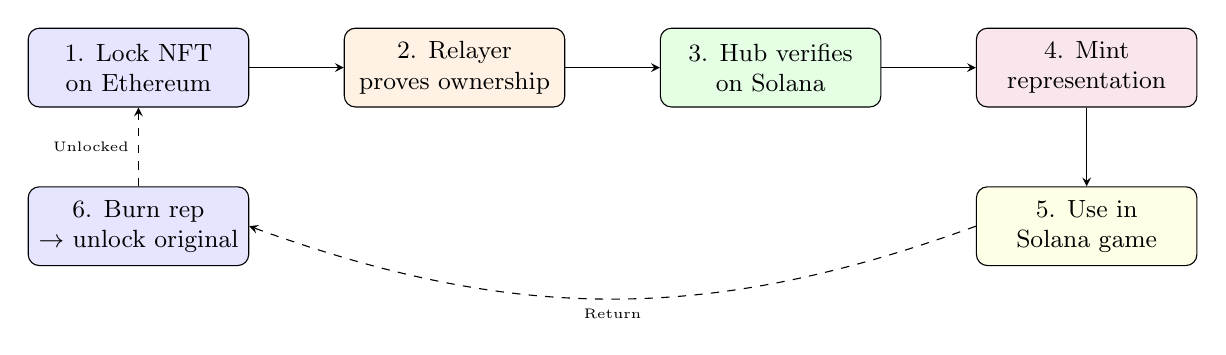
\begin{tikzpicture}[node distance=1.5cm, auto, >=stealth,
    stepbox/.style={rectangle, draw, rounded corners, minimum width=2.8cm, minimum height=1cm, align=center, font=\small}]

    \node (lock)   [stepbox, fill=blue!10]   {1. Lock NFT\\on Ethereum};
    \node (proof)  [stepbox, fill=orange!10, right=1.2cm of lock]  {2. Relayer\\proves ownership};
    \node (verify) [stepbox, fill=green!10,  right=1.2cm of proof] {3. Hub verifies\\on Solana};
    \node (mint)   [stepbox, fill=purple!10, right=1.2cm of verify]{4. Mint\\representation};
    \node (game)   [stepbox, fill=yellow!10, below=1cm of mint]    {5. Use in\\Solana game};
    \node (unlock) [stepbox, fill=blue!10,   below=1cm of lock]    {6. Burn rep\\$\rightarrow$ unlock original};

    \draw [->] (lock) -- (proof);
    \draw [->] (proof) -- (verify);
    \draw [->] (verify) -- (mint);
    \draw [->] (mint) -- (game);
    \draw [->, dashed] (game.west) to[bend left=20] node[below, font=\tiny] {Return} (unlock.east);
    \draw [->, dashed] (unlock) -- (lock) node[midway, left, font=\tiny] {Unlocked};
\end{tikzpicture}
}
\caption{NFT cross chain lifecycle. The original is locked on Ethereum while a provably-linked representation exists on Solana. Burning the Solana representation unlocks the original.}
\end{figure}

The key guarantee: both the original \textit{and} the representation can never be simultaneously active. This is enforced by the ZK proof, not a trusted custodian.

\begin{lstlisting}[language=Java, caption={Solidity: NFT Lock and Proof Emission}]
function lockNFT(
    address nftContract,
    uint256 tokenId,
    uint16 destinationChain,
    bytes32 destinationRecipient
) external {
    // Transfer NFT to gateway vault
    IERC721(nftContract).transferFrom(msg.sender, address(this), tokenId);

    // Emit event for Relayers to prove
    emit NFTLocked(
        ++sequenceNumber,
        msg.sender,
        nftContract,
        tokenId,
        destinationChain,
        destinationRecipient,
        keccak256(abi.encodePacked(nftContract, tokenId))
    );
}
\end{lstlisting}

\subsection{Example 4: Cross-Chain Lending}

\subsubsection{Scenario: Collateral on Ethereum, Borrow on Solana}

Carol holds ETH she does not want to sell, but needs USDC on Solana for trading. Without InterLink she must either sell her ETH or bridge it first---losing custody or paying bridge fees. With InterLink she posts ETH as collateral on Ethereum and borrows USDC directly on Solana.

\begin{enumerate}
    \item Carol locks 10 ETH in the Ethereum Gateway as collateral.
    \item A Relayer generates a proof: ``10 ETH locked; current price \$2,000/ETH = \$20,000 collateral.''
    \item The Solana Hub verifies the proof and records Carol's position.
    \item A Solana lending protocol (e.g., Marginfi) accepts the verified claim and issues Carol up to 75\% LTV = 15,000 USDC.
    \item If ETH price drops below the liquidation threshold, the Hub sends a proof-triggered instruction to the Ethereum Gateway to release collateral.
\end{enumerate}

\begin{table}[H]
\centering
\begin{tabular}{@{}lcc@{}}
\toprule
\textbf{Metric} & \textbf{Manual Bridge} & \textbf{InterLink} \\
\midrule
ETH stays on Ethereum & No & Yes \\
USDC on Solana & After bridge delay & Immediately \\
Collateral security & Trust validators & ZK-proven \\
Liquidation & Manual/slow & Proof-triggered \\
Capital efficiency & $\sim$50\% & $\sim$75\% \\
\bottomrule
\end{tabular}
\caption{Cross-chain lending comparison.}
\end{table}

\subsection{Example 5: Simple Token Transfer (Most Common Case)}

Most users will simply move Token X from Chain A to Chain B. Here is the complete timeline:

\begin{figure}[H]
\centering
\resizebox{0.95\textwidth}{!}{
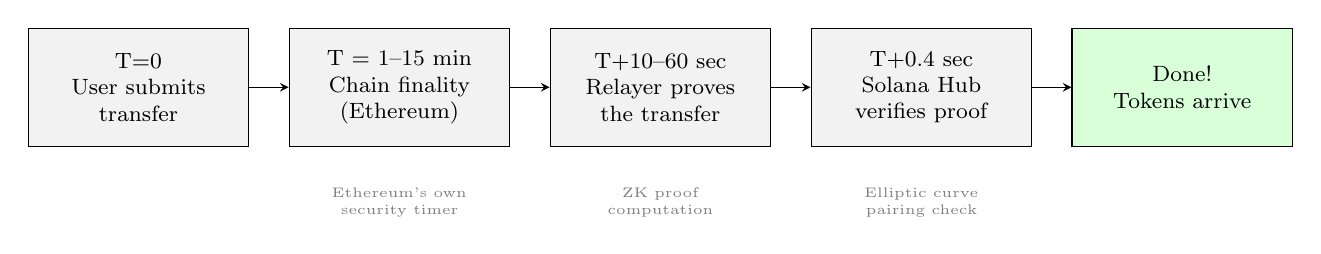
\begin{tikzpicture}[node distance=0.5cm, auto, >=stealth,
    timebox/.style={rectangle, draw, fill=gray!10, minimum width=2.8cm, minimum height=1.5cm, align=center, font=\footnotesize}]

    \node (t0) [timebox] {T=0\\User submits\\transfer};
    \node (t1) [timebox, right=0.5cm of t0] {T = 1--15 min\\Chain finality\\(Ethereum)};
    \node (t2) [timebox, right=0.5cm of t1] {T+10--60 sec\\Relayer proves\\the transfer};
    \node (t3) [timebox, right=0.5cm of t2] {T+0.4 sec\\Solana Hub\\verifies proof};
    \node (t4) [timebox, fill=green!15, right=0.5cm of t3] {Done!\\Tokens arrive};

    \draw [->] (t0) -- (t1);
    \draw [->] (t1) -- (t2);
    \draw [->] (t2) -- (t3);
    \draw [->] (t3) -- (t4);

    \node [below=0.4cm of t1, font=\tiny, text=gray, text width=2.8cm, align=center] {Ethereum's own\\security timer};
    \node [below=0.4cm of t2, font=\tiny, text=gray, text width=2.8cm, align=center] {ZK proof\\computation};
    \node [below=0.4cm of t3, font=\tiny, text=gray, text width=2.8cm, align=center] {Elliptic curve\\pairing check};
\end{tikzpicture}
}
\caption{Timeline for a simple Ethereum $\rightarrow$ Solana transfer. The dominant delay is Ethereum's own finality timer, not InterLink overhead.}
\end{figure}

\textbf{Takeaway:} Total time is 13--20 minutes for Ethereum-sourced transfers---mostly Ethereum's own finality. For faster source chains (Solana, Arbitrum), total time drops to under 2 minutes.

\subsubsection{Developer Integration Guide}

Step 1: Contract Interface
\begin{lstlisting}[language=Java, caption={Solidity: InterLink Integration Interface}]
interface IInterLinkRouter {
    function sendMessage(
        uint16 destinationChain,
        bytes32 recipient,
        bytes calldata payload,
        address feeToken,
        uint256 feeAmount
    ) external payable;
    
    function estimateFee(
        uint16 destinationChain,
        bytes calldata payload
    ) external view returns (uint256);
}
\end{lstlisting}

Step 2: Payload Encoding
Standardized payload format ensures compatibility across chains:

\begin{lstlisting}[language=Rust, caption={Rust: Payload Encoding Standard}]
#[derive(Serialize, Deserialize)]
struct InterLinkPayload {
    version: u8,
    action: ActionType,
    sender: Address,
    recipient: Address,
    data: Vec<u8>,
    deadline: u64,
}

enum ActionType {
    Transfer,
    Swap,
    ContractCall,
    Governance,
}
\end{lstlisting}

Step 3: Error Handling
Implement robust error handling for cross chain operations:

\begin{lstlisting}[language=Java, caption={Solidity: Cross-Chain Error Handling}]
contract CrossChainApp {
    mapping(uint64 => CrossChainTx) public pendingTxs;
    
    function handleExecution(uint64 sequence, bool success, bytes memory result) external {
        CrossChainTx storage tx = pendingTxs[sequence];
        
        if (success) {
            // Process successful execution
            executeCallback(tx.callback, result);
        } else {
            // Handle failure - initiate refund or retry
            initiateRefund(tx);
        }
        
        delete pendingTxs[sequence];
    }
}
\end{lstlisting}

These examples demonstrate how InterLink enables previously impossible cross chain operations, from simple token transfers to complex multi chain DeFi strategies, all with strong guarantees of atomicity, security, and efficiency.


\section{Comparison with State of the Art}
\label{sec:compare}

InterLink competes in a crowded market. However, its architecture offers distinct advantages over incumbents.

\begin{table}[H]
\centering
\footnotesize
\setlength{\tabcolsep}{4pt}
\begin{tabular}{@{}lcccccc@{}}
\toprule
Protocol & Trust Model & Latency & Gas Cost & Finality & Setup & Extensibility \\ \midrule
InterLink & ZK-Light Client & Medium & Low (O(1)) & Src Finality & Trustless & High \\
LayerZero v2 & DVNs (Multi-sig) & Low & Low & Instant & Permissioned & High \\
Axelar & PoS Validators & Medium & Medium & 1-2 mins & Trusted & Medium \\
Wormhole & Guardian Set (19/19) & Low & Low & Instant & Trusted & High \\
Cosmos IBC & Light Client & Low & Low & Instant & Trustless & Low \\ \bottomrule
\end{tabular}
\caption{Comprehensive Competitive Analysis}
\label{tab:comparison_detailed}
\end{table}

\subsection{InterLink vs. LayerZero}

\subsubsection{Technical Architecture Comparison}

LayerZero v2 Overview:
\begin{itemize}
    \item Ultra Light Nodes (ULNs): Permissioned off-chain oracles that attest to cross chain events
    \item Decentralized Verifier Networks (DVNs): External parties that validate message authenticity
    \item Configurable Security: Users choose which DVNs to trust for each message
    \item Modular Design: Separate oracle, relayer, and verification components
\end{itemize}

InterLink Advantages:
\begin{itemize}
    \item Cryptographic Security: ZK proofs provide mathematical guarantees vs. social consensus
    \item Unified Verification: Single proof validates both event and consensus vs. multiple DVN attestations
    \item Trust Minimization: No reliance on external parties for security
    \item Performance: Amortized verification cost scales better with message volume
\end{itemize}

\subsubsection{Economic Comparison}

LayerZero Economics:
\begin{itemize}
    \item Variable fees based on DVN selection and gas prices
    \item Permissioned relayers may extract MEV
    \item Governance controlled by LZ token holders
\end{itemize}

InterLink Economics:
\begin{itemize}
    \item Predictable fees with buy-back-and-burn mechanism
    \item Censorship-resistant relayer network
    \item Quadratic voting ensures fair governance
\end{itemize}

\subsubsection{Security Model Analysis}

LayerZero v2 relies on a "security stack" where users select trusted DVNs. While flexible, this creates:
\begin{itemize}
    \item Trust Assumptions: Users must research and trust multiple external parties
    \item Coordination Risk: All selected DVNs must remain honest simultaneously
    \item Centralization Risk: Popular DVNs become single points of failure
\end{itemize}

InterLink eliminates these assumptions through cryptographic verification, where security derives directly from the source chain's consensus rather than external attestations.

\subsection{InterLink vs. Axelar}

\subsubsection{Consensus Mechanism Differences}

Axelar Network Overview:
\begin{itemize}
    \item Dedicated Blockchain: Axelar runs its own PoS network with 75 validators
    \item Threshold Signatures: Uses MPC-based threshold signatures for cross chain messages
    \item Gateway Contracts: Deployed on supported chains to facilitate message passing
    \item Validator Staking: 75M AXL minimum stake requirement
\end{itemize}

InterLink's Hub-and-Spoke Approach:
\begin{itemize}
    \item Existing High-Performance Chain: Leverages Solana's battle-tested infrastructure
    \item ZK-Based Verification: Cryptographic proofs replace signature-based consensus
    \item Reduced Complexity: No need to bootstrap and secure a new blockchain
    \item Inherited Security: Benefits from Solana's economic security without additional staking requirements
\end{itemize}

\subsubsection{Scalability Analysis}

Axelar's dedicated blockchain creates scalability challenges:
\begin{itemize}
    \item Validator Throughput: Limited by 75 validator consensus
    \item Cross-Chain Latency: Additional consensus round for each message
    \item Upgrade Complexity: Coordinating validator set updates across chains
\end{itemize}

InterLink's architecture scales better:
\begin{itemize}
    \item Hub Throughput: Inherits Solana's 50k+ TPS capacity
    \item Verification Parallelism: ZK proofs can be verified in parallel
    \item Upgrade Flexibility: Protocol upgrades don't require chain consensus
\end{itemize}

\subsection{InterLink vs. Wormhole}

\subsubsection{Guardian Model vs. Relayer Network}

Wormhole Guardian Overview:
\begin{itemize}
    \item Guardian Network: 19 reputable entities that sign cross chain messages
    \item Multi-Signature Verification: Requires 13/19 signatures for validity
    \item Reputation-Based Security: Guardians selected for track record and stake
    \item Centralized Governance: Guardian set controlled by Wormhole foundation
\end{itemize}

InterLink's Decentralized Approach:
\begin{itemize}
    \item Permissionless Relayers: Anyone can participate by staking ILINK
    \item Economic Incentives: Slashing and rewards align relayer behavior
    \item Censorship Resistance: No central authority can prevent message relay
    \item Scalable Security: Security scales with economic stake, not fixed committee size
\end{itemize}

\subsubsection{Risk Analysis}

Wormhole's Guardian model introduces risks:
\begin{itemize}
    \item Coordinator Compromise: If multiple Guardians collude or are coerced
    \item Reputation Gaming: Guardians might prioritize reputation over security
    \item Governance Capture: Foundation control over Guardian selection
\end{itemize}

InterLink mitigates these through:
\begin{itemize}
    \item Cryptographic Security: Invalid proofs are mathematically impossible
    \item Economic Alignment: Relayers lose stake for dishonest behavior
    \item Decentralized Governance: Quadratic voting prevents plutocracy
\end{itemize}

\subsection{InterLink vs. Cosmos IBC}

\subsubsection{Light Client Efficiency Comparison}

IBC Light Client Overview:
\begin{itemize}
    \item Tendermint Light Client: Verifies block headers through validator signatures
    \item Relayer Model: Permissionless relayers submit headers and proofs
    \item Connection Handshake: Requires initial connection establishment between chains
    \item State Verification: Verifies state proofs against verified headers
\end{itemize}

ZK-Enhanced Interoperability:
\begin{itemize}
    \item Compressed Verification: ZK proofs reduce consensus verification from O(n) to O(1)
    \item Universal Compatibility: Works with any consensus mechanism (PoW, PoS, etc.)
    \item Reduced On-Chain Cost: Amortized verification enables cheaper cross chain calls
    \item Unified Interface: Single protocol handles all chain types
\end{itemize}

\subsubsection{Technical Efficiency Gains}

IBC requires on-chain verification of:
\begin{itemize}
    \item Block header validity (validator signatures)
    \item Merkle proof inclusion
    \item State transition correctness
\end{itemize}

InterLink compresses this into a single ZK proof that attests to all three simultaneously, providing:
\begin{itemize}
    \item Reduced Gas Costs: 10-100x lower verification costs on destination chains
    \item Faster Finality: No need to wait for light client updates
    \item Better Privacy: Transaction details can be hidden while proving validity
\end{itemize}

\subsection{Quantitative Performance Comparison}

\subsubsection{Latency Analysis}

\begin{table}[H]
\centering
\begin{tabular}{@{}lcccc@{}}
\toprule
Metric & InterLink & LayerZero & Axelar & Wormhole \\ \midrule
Source Finality & 1-15 min & Instant & 1-2 min & Instant \\
Proof Generation & 10-60 sec & N/A & N/A & N/A \\
Verification & <1 sec & <1 sec & <1 sec & <1 sec \\
Total Latency & 2-16 min & 1-5 min & 2-5 min & 1-3 min \\
\end{tabular}
\caption{Latency Comparison Across Protocols}
\end{table}

\subsubsection{Cost Efficiency Analysis}

InterLink achieves superior cost efficiency through:
\begin{itemize}
    \item Batching: 100-message batches reduce per-message costs by 99\%
    \item Recursive Proofs: Aggregate proofs across multiple messages
    \item Amortized Verification: O(1) verification regardless of message complexity
\end{itemize}

\subsubsection{Security Quantification}

\begin{table}[H]
\centering
\begin{tabular}{@{}lccc@{}}
\toprule
Security Property & InterLink & Competitors & Advantage \\ \midrule
Cryptographic Security & $\checkmark$ & $\times$ & Mathematical guarantees \\
Censorship Resistance & $\checkmark$ & $\times$ & Permissionless relayers \\
Economic Alignment & $\checkmark$ & Partial & Slashing + rewards \\
Scalable Security & $\checkmark$ & $\times$ & Stake-based, not committee \\
\end{tabular}
\caption{Security Feature Comparison}
\end{table}

\subsection{Unique InterLink Advantages}

\subsubsection{Innovative Features}

Unified Liquidity Layer:
\begin{itemize}
    \item Aggregates liquidity across all connected chains
    \item Enables atomic cross chain swaps with optimal routing
    \item Provides unified price discovery and arbitrage opportunities
\end{itemize}

Recursive Proof Composition:
\begin{itemize}
    \item Enables proof aggregation across multiple messages
    \item Supports complex multi-step cross chain operations
    \item Maintains succinctness even for batched operations
\end{itemize}

Economic Sustainability:
\begin{itemize}
    \item Buy-back-and-burn creates deflationary token dynamics
    \item Quadratic governance prevents plutocratic capture
    \item Stake-weighted security scales with adoption
\end{itemize}

\subsubsection{Market Positioning}

InterLink positions itself as the "ZK-native interoperability layer" that combines:
\begin{itemize}
    \item Trustless Security: Cryptographic guarantees eliminate bridge risks
    \item Developer Experience: Simple APIs for complex cross chain operations
    \item Economic Efficiency: Low costs and sustainable token economics
    \item Future-Proofing: Extensible architecture for emerging use cases
\end{itemize}

This comprehensive analysis demonstrates that InterLink offers a superior combination of security, efficiency, and extensibility compared to existing interoperability solutions, positioning it as the foundation for the next generation of cross chain applications.

\section{Limitations and Known Trade-offs}
\label{sec:limitations}

Any honest research paper must acknowledge its limitations. InterLink is a significant improvement over existing bridges, but it is not a perfect solution to every problem. This section enumerates the current limitations, the reasons for each trade-off, and how we plan to address them.

\subsection{Latency: Source-Chain Finality is the Bottleneck}

\textbf{Limitation:} Cross-chain transfers are only as fast as the source chain's finality. For Ethereum mainnet, this is 12--15 minutes. InterLink cannot speed this up.

\textbf{Why:} The entire security model depends on proving events that are \textit{final}---meaning they cannot be reorganized away. Accepting events before finality would expose InterLink to double-spend attacks on the source chain. This is a deliberate and necessary trade-off.

\textbf{Mitigation:} For Layer 2 chains (Arbitrum, Optimism) and fast chains (Solana, Cosmos), finality is seconds to minutes, reducing total transfer time to under 2 minutes. We also plan to explore ``optimistic relay'' modes for low-value transfers where speed outweighs maximum security.

\subsection{Proof Generation Compute Cost}

\textbf{Limitation:} Generating a zk-SNARK proof requires significant CPU time (currently $\sim$850ms on consumer hardware, $\sim$100ms on server-grade hardware). This means Relayers need real computing infrastructure.

\textbf{Why:} ZK proof generation involves polynomial evaluations, Multi-Scalar Multiplications (MSMs), and Fast Fourier Transforms (FFTs)---these are mathematically expensive by design. The cost is what makes the proof secure.

\textbf{Mitigation:} We are actively researching GPU and FPGA acceleration (see Section~\ref{sec:status}), which can reduce proving time by 10--100$\times$. Distributed proving pools can also distribute the compute load across many machines.

\subsection{Trusted Setup for KZG (Ethereum-side)}

\textbf{Limitation:} The KZG polynomial commitment scheme used for Ethereum-side verification requires a one-time ``trusted setup'' ceremony to generate Structured Reference Strings (SRS). If all participants in the ceremony collude, they could forge proofs.

\textbf{Why:} KZG provides constant-size proofs (48 bytes) and constant-time verification, which is critical for affordable Ethereum gas costs. The alternative (IPA) is transparent but slower to verify on-chain.

\textbf{Mitigation:} We will participate in or reference Ethereum's Ceremony (Powers of Tau), which involves thousands of participants. The probability of all participants colluding is negligible. Long-term, we are evaluating transparent alternatives like STARKs for a future trusted-setup-free design.

\begin{table}[H]
\centering
\begin{tabular}{@{}lcc@{}}
\toprule
\textbf{Scheme} & \textbf{Proof Size} & \textbf{Trusted Setup?} \\
\midrule
KZG (current EVM side) & 48 bytes & Yes (Powers of Tau) \\
IPA (current recursion) & $O(\log n)$ bytes & No \\
STARK (future) & $\sim$100 KB & No \\
\bottomrule
\end{tabular}
\caption{Comparison of commitment schemes. InterLink uses KZG where verification cost matters most and IPA where setup-freedom matters.}
\end{table}

\subsection{Hub Availability: Solana Dependency}

\textbf{Limitation:} InterLink's Hub runs on Solana. If Solana experiences an outage (it has historically), cross chain transfers are paused.

\textbf{Why:} We chose Solana for its 50,000+ TPS throughput and sub-400ms block times---essential for a high performance coordination hub. A decentralized multi-hub design is more complex and introduces coordination overhead.

\textbf{Mitigation:}
\begin{itemize}
    \item \textit{Proof queue persistence:} Relayer proofs are queued during outages and submitted when Solana recovers. No funds are lost; transfers are delayed.
    \item \textit{Multi-hub failover (roadmap):} We plan to deploy secondary hubs on Arbitrum and Cosmos Hub as fallbacks.
    \item \textit{Asset safety during outages:} User assets are always in the source chain Gateway vault. They cannot be lost during Hub downtime.
\end{itemize}

\subsection{Relayer Liveness}

\textbf{Limitation:} If no Relayer processes a message (e.g., if all Relayers go offline), the transfer stalls. This is a liveness risk, not a safety risk---funds are never lost, but transfers may be delayed.

\textbf{Why:} The permissionless model means anyone can run a Relayer but nobody is \textit{required} to. We solve this through economic incentives (Relayers earn fees) but can't force participation.

\textbf{Mitigation:}
\begin{itemize}
    \item The DAO can activate ``emergency relaying subsidies'' to incentivize participation during low-activity periods.
    \item A multi-relayer submission model means any one of hundreds of Relayers can process each message.
    \item Users can run their own Relayer for self-sovereign transfers.
\end{itemize}

\subsection{Limited Chain Support at Launch}

\textbf{Limitation:} InterLink v1 supports Ethereum and Solana only. Adding new chains requires deploying Gateway contracts, writing chain-specific ZK circuits, and completing audits.

\textbf{Why:} Each chain has a unique consensus mechanism (BLS-12-381 for Ethereum, Ed25519 for Cosmos, etc.), requiring custom circuit implementations. Security audits for each circuit take months.

\textbf{Roadmap:} See Section~\ref{sec:status} for the phased multi chain expansion plan. Arbitrum and Cosmos Hub are the next priority targets (Q4 2027).

\subsection{Summary of Trade-offs}

\begin{table}[H]
\centering
\begin{tabular}{@{}lccl@{}}
\toprule
\textbf{Limitation} & \textbf{Safety Risk?} & \textbf{Liveness Risk?} & \textbf{Mitigation} \\
\midrule
Ethereum finality delay & No & No & Faster chains = faster transfers \\
Proof generation time & No & Partial & GPU/FPGA acceleration \\
KZG trusted setup & Negligible & No & Powers of Tau ceremony \\
Solana Hub downtime & No & Yes & Proof queuing; multi-hub fallback \\
Relayer liveness & No & Yes & Economic incentives; DAO subsidies \\
Limited chain support & No & No & Phased expansion roadmap \\
\bottomrule
\end{tabular}
\caption{Summary of InterLink limitations and mitigations. Importantly, \textbf{no limitation poses a safety risk}---user funds are never at risk from these constraints.}
\end{table}

\section{Conclusion}

We began this paper with a simple observation: the multi chain world is fragmented, and fragmentation is expensive. Over \$2 billion stolen from bridges. Billions more in capital trapped in isolated ecosystems. Users forced to trust anonymous validator committees with their savings.

InterLink's answer is as simple as it is powerful: \textbf{replace trust with proof}.

By combining Halo2 zk-SNARKs with Solana's high performance execution, InterLink provides what was previously considered an unsolvable trilemma:

\begin{itemize}
    \item \textbf{Trustlessness} of a full light client---without its cost.
    \item \textbf{Cost-efficiency} of a multisig bridge---without its security risks.
    \item \textbf{Scalability} through recursive proof folding---O(1) verification for any batch size.
\end{itemize}

The protocol is not just a bridge. It is a \textit{unified liquidity layer}---a substrate on which developers can build cross chain applications that feel native, where users never worry about which chain holds their assets. This is what ``Chain Abstraction'' looks like in practice: InterLink doing the hard work invisibly in the background.

We are at the beginning of this journey. Ethereum$\leftrightarrow$Solana in 2027. Multi-chain in 2028. Universal in the years beyond. We invite the cryptography community to audit our circuits, developers to build on our SDK, and researchers to push the boundaries of what ZK proofs can verify.

The future of blockchains is not a winner-take-all race. It is a cooperative ecosystem where every chain speaks the same language of verifiable math. InterLink is that language.

\vspace{0.3in}
\textit{Source code, circuit implementations, and technical documentation available at:}\\
\url{https://github.com/MeridianAlgo/Interlink}

\subsection{Future Work and Research Directions}

Our roadmap encompasses multiple research vectors that will enhance InterLink's capabilities and expand its applicability across the blockchain ecosystem.

\subsubsection{Cryptographic Enhancements}

Zero-Knowledge Virtual Machines (zkVMs):
\begin{itemize}
    \item Universal Circuit Templates: Develop standardized circuit templates for common operations (ERC20 transfers, DEX swaps, NFT minting)
    \item Recursive Proof Aggregation: Implement advanced recursive structures for aggregating proofs across multiple chains simultaneously
    \item Post-Quantum Security: Research quantum-resistant proof systems to future-proof against cryptographic advances
    \item Multi-Party Computation Integration: Combine MPC with ZK proofs for enhanced privacy and scalability
\end{itemize}

Privacy-Preserving Interoperability:
\begin{itemize}
    \item Zero-Knowledge Token Transfers: Enable cross chain transfers where amount and recipient remain hidden
    \item Confidential DEX Operations: Private order matching and execution across chains
    \item Anonymous Governance: Quadratic voting with privacy preservation
    \item Mixed ZK Protocols: Integration with Aztec, Tornado Cash, and other privacy-focused systems
\end{itemize}

\subsubsection{Performance and Scalability Improvements}

Hardware Acceleration Research:
\begin{itemize}
    \item FPGA Implementation: Custom FPGA designs optimized for Halo2 proving operations
    \item ASIC Development: Application-specific integrated circuits for high throughput proof generation
    \item GPU Optimization: CUDA implementations for parallel proof computation
    \item Distributed Proving Networks: Decentralized proving pools for horizontal scaling
\end{itemize}

Network Layer Optimizations:
\begin{itemize}
    \item Proof Compression: Advanced compression techniques to reduce proof sizes by 10-100x
    \item Batching Algorithms: Sophisticated batching strategies for optimal gas utilization
    \item Layer 2 Integration: Direct integration with rollups and sidechains for reduced latency
    \item Cross-Chain State Channels: Payment channel networks spanning multiple blockchains
\end{itemize}

\subsubsection{Ecosystem Expansion}

Multi-Chain Support Roadmap:
\begin{itemize}
    \item Layer 1 Integration: Bitcoin, Ethereum, Solana, Cosmos, Polkadot, Avalanche, Near
    \item Layer 2 Support: Optimism, Arbitrum, Polygon, zkSync, StarkNet, Scroll
    \item Altchain Compatibility: Monero (privacy), Algorand (speed), Flow (NFTs)
    \item Enterprise Chains: Hyperledger, Quorum, Corda integration
\end{itemize}

DeFi and NFT Primitives:
\begin{itemize}
    \item Cross-Chain Lending: Atomic borrowing and lending across protocols
    \item Unified Liquidity Pools: Aggregated liquidity from Uniswap, SushiSwap, PancakeSwap
    \item NFT Fractionalization: Cross-chain NFT ownership and trading
    \item Derivatives Markets: Cross-chain options, futures, and synthetic assets
\end{itemize}

\subsubsection{Developer Experience and Tooling}

SDK and Framework Development:
\begin{itemize}
    \item InterLink SDK: Unified APIs for cross chain application development
    \item Smart Contract Libraries: Pre-built contracts for common cross chain patterns
    \item Testing Frameworks: Simulation environments for cross chain application testing
    \item Deployment Tools: Automated deployment and configuration management
\end{itemize}

Integration and Interoperability Standards:
\begin{itemize}
    \item Cross-Chain Standards: Standardized message formats and protocol interfaces
    \item Oracle Networks: Decentralized price feeds and data oracles across chains
    \item Identity Systems: Cross-chain digital identity and reputation
    \item Governance Frameworks: Interoperable DAO structures and voting mechanisms
\end{itemize}

\subsubsection{Long-Term Research Vision}

Fractal Scaling Architecture:
\begin{itemize}
    \item L3 Application Chains: App-specific chains settling to InterLink as DA layer
    \item Recursive Interoperability: Chains that can themselves be InterLink hubs
    \item Meta-Protocol Layer: Higher-order protocols built on InterLink infrastructure
    \item Quantum-Resistant Upgrades: Migration paths for post-quantum cryptography
\end{itemize}

Societal Impact Research:
\begin{itemize}
    \item Global Financial Inclusion: Cross-border payments for unbanked populations
    \item Digital Sovereignty: User-owned identity and assets across jurisdictions
    \item Decentralized Governance: Global decision-making without geographic boundaries
    \item Economic Mobility: Reduced friction in international trade and commerce
\end{itemize}

\subsubsection{Research Collaboration Opportunities}

We actively seek partnerships with:
\begin{itemize}
    \item \textit{Academic Institutions:} Cryptography research, formal verification, distributed systems
    \item \textit{Industry Partners:} Hardware manufacturers, DeFi protocols, Layer 1 platforms
    \item \textit{Government Entities:} Regulatory compliance, cross-border payment frameworks
    \item \textit{NGOs and Impact Organizations:} Financial inclusion and digital sovereignty initiatives
\end{itemize}

\subsubsection{Risks, Mitigations \& Contingency Planning}

\textit{Technical Risks:}
\begin{itemize}
    \item \textit{Cryptographic Breaks:} Transition to Post-Quantum Signature (PQC) circuits if required. Continuous auditing by Trail of Bits.
    \item Liveness Failure: If relayers halt, governance can temporarily subsidize proves or slash idle bonded relayers to restore service.
    \item Solana Congestion: Adaptive message prioritization and multi chain hub failovers (e.g. Arbitrum Hub fallback).
\end{itemize}

\textit{Economic \& Adoption Risks:}
\begin{itemize}
    \item \textit{Vaporware Accusations:} Countered by public PoC benchmarks and open-source SDK repositories.
    \item \textit{Liquidity Fragmentation:} Incentives for LPs to bridge via ILINK to unify states.
\end{itemize}

All source code, circuit implementations, and documentation are open-source and available at \url{https://github.com/MeridianAlgo/Interlink}.

\newpage

\section*{Glossary}
\addcontentsline{toc}{section}{Glossary}

For readers unfamiliar with blockchain and cryptography terminology, this glossary provides plain-English definitions.

\begin{description}[style=nextline, leftmargin=3cm, labelwidth=2.8cm]

\item[Accumulator] A cryptographic object that ``collects'' multiple proofs into one. Think of it like a zip file for proofs---many inputs, one compressed output.

\item[BLS Signature] A type of digital signature that multiple people can combine into one. If 100 people sign a document, you get one combined signature instead of 100 separate ones. Ethereum uses this for validator consensus.

\item[Bridge] Software that moves assets between blockchains. Traditional bridges use trusted validators; InterLink uses math.

\item[Circuit] A mathematical representation of computation that can be proven with zero knowledge. Like a blueprint that says ``if inputs satisfy these rules, output is valid.''

\item[Commitment] A cryptographic ``sealed envelope'' that hides data while proving you can't change it later. You commit to a value without revealing it.

\item[Consensus] Agreement among network participants about the state of the blockchain. Different chains use different consensus mechanisms (PoW, PoS, etc.).

\item[CPI (Cross-Program Invocation)] Solana's way of letting one program call another. Like a function calling a library in traditional programming.

\item[DEX (Decentralized Exchange)] A trading platform that runs on blockchain without a central company. Examples: Uniswap, Jupiter.

\item[Elliptic Curve] A mathematical structure used in modern cryptography. Points on special curves enable secure digital signatures and commitments.

\item[Finality] The point when a blockchain transaction becomes irreversible. Ethereum reaches finality in ~15 minutes; Solana in ~400ms.

\item[Gas / Compute Units] The ``fuel'' that powers blockchain transactions. Users pay gas fees to compensate validators for processing.

\item[Gateway Contract] InterLink's ``embassy'' on each blockchain. It holds assets, emits events, and executes verified messages.

\item[Halo2] A zero knowledge proof system developed by Zcash. InterLink uses it because it doesn't require a trusted setup for internal proofs.

\item[Hub] InterLink's central coordinator on Solana. All cross chain messages route through the Hub.

\item[IPA (Inner Product Argument)] A mathematical technique for proving polynomial evaluations. Used in Halo2 for efficient recursive proofs.

\item[KZG Commitment] A way to commit to data using elliptic curve pairings. Provides constant-size proofs but requires trusted setup.

\item[Light Client] Software that verifies blockchain data without storing the full chain. InterLink's ZK circuits act as ``light clients in a proof.''

\item[Merkle Proof] A cryptographic proof that data exists in a larger set. Used to prove a transaction is included in a block without showing all transactions.

\item[Multisig] A wallet requiring multiple signatures to authorize transactions. Traditional bridges use multisigs, which are vulnerable to collusion.

\item[Pairing] A mathematical operation on elliptic curves that enables advanced cryptography. Used for BLS signatures and KZG commitments.

\item[PDA (Program Derived Address)] A Solana address controlled by a program rather than a private key. Useful for program-owned accounts.

\item[Proof] In ZK systems, a short piece of data that convinces a verifier a statement is true without revealing the underlying evidence.

\item[Prover] The entity generating ZK proofs. In InterLink, Relayers are provers.

\item[Recursion] A proof that verifies other proofs. Enables compressing many proofs into one.

\item[Relayer] An InterLink node that watches for events, generates proofs, and submits them to the Hub.

\item[Slashing] Punishing misbehaving validators by destroying part of their staked tokens.

\item[SNARK] Succinct Non-interactive Argument of Knowledge. A type of ZK proof that is small and fast to verify.

\item[Spoke] Any blockchain connected to InterLink's Hub. Ethereum, Arbitrum, Cosmos are all ``spokes.''

\item[Staking] Locking tokens as collateral to participate in network operations. Relayers stake ILINK to prove honesty.

\item[Verifier] The entity checking proofs. In InterLink, the Solana Hub is the verifier.

\item[Witness] Private inputs to a ZK circuit. The prover knows the witness; the verifier only sees the proof.

\item[Zero-Knowledge] A proof that reveals nothing except that a statement is true. The verifier learns the conclusion without the evidence.

\item[zk-SNARK] Zero-Knowledge Succinct Non-interactive Argument of Knowledge. The specific proof system InterLink uses.

\end{description}

\newpage

\begin{thebibliography}{99}
\addcontentsline{toc}{section}{References}

\bibitem{halo2}
Electric Coin Co. \textit{The Halo2 Proving System}. 2024. \url{https://zcash.github.io/halo2/}

\bibitem{plonk}
Gabizon, A., Williamson, Z., Ciobotaru, O. \textit{PLONK: Permutations over Lagrange-bases for Oecumenical Noninteractive arguments of Knowledge}. ePrint 2019/953.

\bibitem{pasta}
ECC \& Zcash Foundation. \textit{The Pasta Curves for Halo 2 and Beyond}. 2021.

\bibitem{solana}
Yakovenko, A. \textit{Solana: A new architecture for a high performance blockchain}. 2018.

\bibitem{layerzero}
Zarick, R., et al. \textit{LayerZero: Trustless Omnichain Interoperability Protocol}. 2021.

\bibitem{kzg}
Kate, A., Zaverucha, G.M., Goldberg, I. \textit{Constant-Size Commitments to Polynomials and Their Applications}. ASIACRYPT 2010.

\bibitem{wormhole}
Wormhole Team. \textit{Wormhole: Generic Message Passing}. 2020.

\bibitem{bitcoin}
Nakamoto, S. \textit{Bitcoin: A Peer-to-Peer Electronic Cash System}. 2008.

\bibitem{ethereum}
Buterin, V. \textit{A Next-Generation Smart Contract and Decentralized Application Platform}. 2014.

\bibitem{zcash}
Hopewood, D., et al. \textit{Zcash Protocol Specification}. 2023.

\bibitem{recursive}
Valiant, P. \textit{Incrementally Verifiable Computation or The Power of Memory from Self-Reference}. 2008.

\bibitem{groth16}
Groth, J. \textit{On the Size of Pairing-based Non-interactive Zero-knowledge Proofs}. 2016.

\bibitem{bulletproofs}
Bunz, B., et al. \textit{Bulletproofs: Short Proofs for Confidential Transactions and More}. 2018.

\bibitem{stark}
Ben-Sasson, E., et al. \textit{Scalable, Transparent, and Post-Quantum Secure Computational Integrity}. 2018.

\bibitem{axelar}
Axelar Team. \textit{Axelar Network: Connecting Applications with Blockchain Ecosystems}. 2021.

\bibitem{ibc}
Goes, C. \textit{The Inter-blockchain Communication Protocol}. 2020.

\bibitem{pos}
King, S., Nadal, S. \textit{Peercoin: Peer-to-Peer Crypto-Currency with Proof-of-Stake}. 2012.

\bibitem{casper}
Buterin, V., Griffith, V. \textit{Casper the Friendly Finality Gadget}. 2017.

\bibitem{tendermint}
Buchman, E. \textit{Tendermint: Software You Can Trust}. 2016.

\bibitem{avalanche}
Rocket, T., et al. \textit{Scalable and Probabilistic Leaderless Byzantine Fault Tolerance: The Avalanche Protocol Family}. 2019.

\bibitem{fiat-shamir}
Fiat, A., Shamir, A. \textit{How to Prove Yourself: Practical Solutions to Identification and Signature Problems}. 1986.

\bibitem{mimc}
Albrecht, C., et al. \textit{MiMC: Efficient Encryption and Hashing with Ultra-Low Multiplicative Complexity}. 2016.

\bibitem{poseidon}
Grassi, L., et al. \textit{Poseidon: A New Hash Function for Zero-Knowledge Proof Systems}. 2021.

\bibitem{merkle}
Merkle, R. \textit{A Digital Signature Based on Conventional Encryption}. 1987.

\bibitem{polkadot}
Wood, G. \textit{Polkadot: Vision for a Heterogeneous Multi-chain Framework}. 2016.

\bibitem{algorand}
Micali, S. \textit{Algorand: The Efficient and Democratic Ledger}. 2016.

\bibitem{cosmos}
Kwon, J., Buchman, E. \textit{Cosmos: A Network of Distributed Ledgers}. 2016.

\bibitem{bip32}
Wuille, P. \textit{Hierarchical Deterministic Wallets}. BIP 32, 2012.

\bibitem{sui}
Sui Team. \textit{Sui Blockchain: High Throughput and Low Latency}. 2022.

\bibitem{aptos}
Aptos Team. \textit{The Aptos Blockchain: Safe, Scalable, and Upgradeable Layer 1}. 2022.

\bibitem{rollup}
Buterin, V. \textit{An Incomplete Guide to Rollups}. 2021.

\bibitem{data-availability}
Al-Bassam, M., et al. \textit{Fraud and Data Availability Proofs: Maximising Light Client Security and Scaling Blockchains with Dishonest Majorities}. 2018.

\bibitem{celestia}
Celestia Team. \textit{Celestia: A Lazy Ledger for dApps}. 2021.

\bibitem{eigenlayer}
Sreeram, K., et al. \textit{EigenLayer: The Restaking Collective}. 2023.

\bibitem{flashbots}
Daian, P., et al. \textit{Flash Boys 2.0: Frontrunning in Decentralized Exchanges, Miner Extractable Value, and Transaction Ordering in Next-Generation Ethereum}. 2019.

\bibitem{uniswap}
Adams, H., et al. \textit{Uniswap v3 Core}. 2021.

\bibitem{curve}
Egorov, M. \textit{StableSwap - efficient mechanism for Stablecoin liquidity}. 2019.

\bibitem{chainlink}
Ellis, S., et al. \textit{Chainlink: A Decentralized Oracle Network}. 2017.

\bibitem{makerdao}
MakerDAO Team. \textit{The Maker Protocol: Whitepaper}. 2020.

\bibitem{aave}
Aave Team. \textit{Aave Protocol: Smart Contract Based Decentralized Lending and Borrowing}. 2020.

\bibitem{compound}
Leshner, R., Hayes, G. \textit{Compound: The Money Market Protocol}. 2019.

\bibitem{monero}
van Saberhagen, N. \textit{CryptoNote v2.0}. 2013.

\bibitem{quadratic-voting}
Lalley, S. P., Weyl, E. G. \textit{Quadratic Voting: How Mechanism Design Can Radicalize Democracy}. 2018.

\bibitem{hyperledger}
Cachin, C. \textit{Architecture of the Hyperledger Blockchain Fabric}. 2016.

\bibitem{libfabric}
Bohra, A., et al. \textit{Interoperating Blockchains}. 2018.

\bibitem{bridging-survey}
Belchior, R., et al. \textit{A Survey on Blockchain Interoperability: Past, Present, and Future}. 2021.

\bibitem{cross chain-sec}
Zia, T., et al. \textit{A Security Analysis of Cross-Chain Bridges}. 2022.

\bibitem{formal-verification}
Bhargavan, K., et al. \textit{Formal Verification of Smart Contracts: Short Paper}. 2016.

\bibitem{rust-safety}
Jung, R., et al. \textit{RustBelt: Securing the Foundations of the Rust Programming Language}. 2017.

\bibitem{zero knowledge-tax}
Goldwasser, S., Micali, S., Rackoff, C. \textit{The Knowledge Complexity of Interactive Proof Systems}. 1985.

\end{thebibliography}

\end{document}
